\documentclass[12pt, a4paper]{article}
\usepackage{../../../myconfig} % Gọi file cấu hình từ ngoài gốc vào

% ==========================================
% BẮT ĐẦU NỘI DUNG TÀI LIỆU
% ==========================================
\begin{document}

% Truyền 3 tham số: {Nhãn cam} {Chữ to chính giữa} {Chữ ở góc phải Header}
\titlebox{Chủ đề: Hàm số}{Tổng hợp câu hỏi hàm số}{Hàm số}


\questionTrueFalse{0}{1}{Cho hàm số \( y = f(x) = x^3 + 3x^2 - 3x + 1 \). Xét tính đúng sai của các mệnh đề sau:}{
    \textbf{a)} & Hàm số trên có hai cực trị gồm một cực tiểu và một cực đại.
    & \textcolor{amberorange}{$\bigcirc$} & \textcolor{amberorange}{$\bigcirc$} \\ \hline
    
    \textbf{b)} & Giá trị lớn nhất của hàm số trên đoạn \([-1; 2]\) bằng 12.
    & \textcolor{amberorange}{$\bigcirc$} & \textcolor{amberorange}{$\bigcirc$} \\ \hline
    
    \textbf{c)} & Hàm số nghịch biến trên khoảng \((-2; -1)\).
    & \textcolor{amberorange}{$\bigcirc$} & \textcolor{amberorange}{$\bigcirc$} \\ \hline
    
    \textbf{d)} & Đạo hàm của hàm số là \(f'(x) = x^2 + 6x - 3\).
    & \textcolor{amberorange}{$\bigcirc$} & \textcolor{amberorange}{$\bigcirc$} \\
}

\questionTrueFalse{0}{2}{Chi phí vận hành trung bình (tính bằng triệu đồng/chuyến) của một công ty vận tải khi vận hành \( x \) chuyển xe mỗi ngày được cho bởi hàm số  
\(A(x) = 0,2x + 2 + \dfrac{500}{x}\)
với \( 10 \leq x \leq 100 \).}{
    \textbf{a)} & Đạo hàm của hàm chi phí trung bình là  
    \(A'(x) = \dfrac{0,2x^2 + 500}{x^2}.\)
    & \textcolor{amberorange}{$\bigcirc$} & \textcolor{amberorange}{$\bigcirc$} \\ \hline
    
    \textbf{b)} & Chi phí trung bình trên mỗi chuyến xe thấp nhất là 22 triệu.
    & \textcolor{amberorange}{$\bigcirc$} & \textcolor{amberorange}{$\bigcirc$} \\ \hline
    
    \textbf{c)} & Nếu do giới hạn về số lượng tài xế khiến công ty chỉ có thể vận hành tối đa 40 chuyến xe mỗi ngày. Chi phí trung bình cho mỗi chuyến xe trong trường hợp này thấp nhất bằng 22,5 triệu đồng.
    & \textcolor{amberorange}{$\bigcirc$} & \textcolor{amberorange}{$\bigcirc$} \\ \hline
    
    \textbf{d)} & Tổng chi phí vận hành của công ty vận tải trong một ngày thấp nhất là 1,1 tỉ đồng.
    & \textcolor{amberorange}{$\bigcirc$} & \textcolor{amberorange}{$\bigcirc$} \\
}

\questionTrueFalse{0}{3}{Đồ thị của hàm số \( y = ax + b + \dfrac{c}{x + d} \) là hình dưới đây

\begin{center}
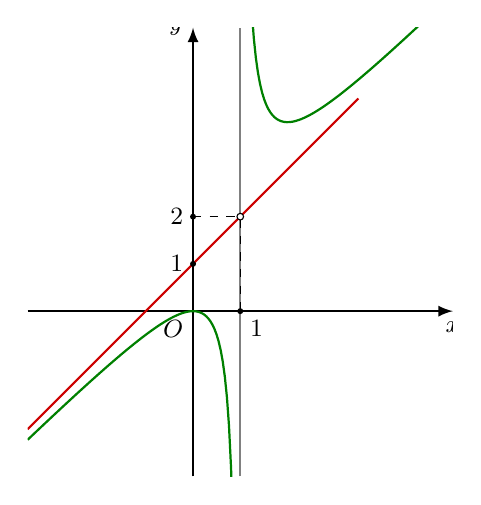
\begin{tikzpicture}[scale=0.6, >=latex]
    
    \clip (-3.5, -3.5) rectangle (5.5, 6);
    % 2. Vẽ hệ trục tọa độ Oxy
    \draw[->, thick] (-3.5, 0) -- (5.5, 0) node[below] {\small $x$};
    \draw[->, thick] (0, -3.5) -- (0, 6) node[left] {\small $y$};
    \node[below left] at (0,0) {\small $O$};

    % 3. Đường tiệm cận đứng x = 1 (màu xám)
    \draw[gray, thick] (1, -3.5) -- (1, 6);

    % 4. Đường tiệm cận xiên y = x + 1 (màu đỏ)
    \draw[thick, red!80!black, domain=-3.5:3.5] plot (\x, {\x + 1});

    % 5. Đồ thị hàm số y = x + 1 + 1/(1 - x) (màu xanh lá)
    % Nhánh trái (x < 1)
    \draw[thick, green!50!black, domain=-3.5:0.85, samples=100] 
        plot (\x, {\x + 1 - 1/(1 - \x)});
    % Nhánh phải (x > 1)
    \draw[thick, green!50!black, domain=1.2:5.5, samples=100] 
        plot (\x, {\x + 1 - 1/(1 - \x)});

    % 6. Các đường dóng nét đứt và điểm đặc biệt
    \draw[dashed] (0, 2) -- (1, 2) -- (1, 0);

    % Các điểm đánh dấu
    \fill[black] (0, 1) circle (1.8pt) node[left] {\small $1$};
    \fill[black] (0, 2) circle (1.8pt) node[left] {\small $2$};
    \fill[black] (1, 0) circle (1.8pt) node[below right] {\small $1$};
    
    % Điểm giao nhau giữa tiệm cận xiên và tiệm cận đứng (1;2)
    \draw[fill=white, draw=black] (1, 2) circle (2pt);
\end{tikzpicture}
\end{center}
}{
    \textbf{a)} & Hàm số nghịch biến trên khoảng \((0;1)\).
    & \textcolor{amberorange}{$\bigcirc$} & \textcolor{amberorange}{$\bigcirc$} \\ \hline
    
    \textbf{b)} & \( \lim\limits_{x \to 1^+} y = -\infty. \)
    & \textcolor{amberorange}{$\bigcirc$} & \textcolor{amberorange}{$\bigcirc$} \\ \hline
    
    \textbf{c)} & Phương trình đường tiệm cận xiên của đồ thị hàm số là:  
    \( y = x + 1. \)
    & \textcolor{amberorange}{$\bigcirc$} & \textcolor{amberorange}{$\bigcirc$} \\ \hline
    
    \textbf{d)} & Tổng \( a + b + c + d = 2. \)
    & \textcolor{amberorange}{$\bigcirc$} & \textcolor{amberorange}{$\bigcirc$} \\
}

\questionTrueFalse{0}{4}{Một cây cầu bắc qua sông có dạng cung \( OA \) của đồ thị hàm số \( y = 4,8 \sin \frac{x}{9} \) và được mô tả trong hệ trục tọa độ với đơn vị trục là mét như hình vẽ. Trục \( Ox \) nằm trên mặt nước sông.

\begin{center}
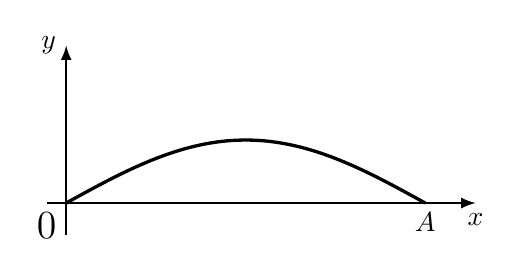
\begin{tikzpicture}[scale=0.8, >=latex]
    % 1. Trục tọa độ Oxy
    \draw[->, thick] (-0.3, 0) -- (6.5, 0) node[below] {$x$};
    \draw[->, thick] (0, -0.5) -- (0, 2.5) node[left] {$y$};

    % 2. Nhãn gốc tọa độ O và điểm A
    \node[below left] at (0, 0) {\Large $0$};
    \node[below] at (5.7, 0) {$A$};

    % 3. Cung cầu hình sin/parabol
    \draw[very thick, domain=0:5.7, samples=100] 
        plot (\x, {1*sin(\x*180/5.7)});
\end{tikzpicture}
\end{center}
}{
    \textbf{a)} & Một sà lan Y chở khối hàng hóa được xếp thành hình hộp chữ nhật với chiều rộng của khối hàng hóa đó là 9 m sao cho sà lan có thể đi qua được gầm cầu. Chiều cao của khối hàng hóa đó phải nhỏ hơn 4,1 m ( kết quả làm tròn đến hàng phần mười ).
    & \textcolor{amberorange}{$\bigcirc$} & \textcolor{amberorange}{$\bigcirc$} \\ \hline
    
    \textbf{b)} & Điểm cao nhất của cây cầu cách mặt nước sông là 1 m.
    & \textcolor{amberorange}{$\bigcirc$} & \textcolor{amberorange}{$\bigcirc$} \\ \hline
    
    \textbf{c)} & Một sà lan X chở khối hàng hóa được xếp thành hình hộp chữ nhật với độ cao 3,6 m so với mực nước sông sao cho sà lan có thể đi qua được gầm cầu. Khi đó chiều rộng của khối hàng hóa đó phải nhỏ hơn 13,01 m ( kết quả làm tròn đến hàng phần trăm ).
    & \textcolor{amberorange}{$\bigcirc$} & \textcolor{amberorange}{$\bigcirc$} \\ \hline
    
    \textbf{d)} & Giả sử chiều rộng của con sông là độ dài đoạn thẳng \( OA \). Chiều rộng con sông là 28,3 m ( kết quả làm tròn đến hàng phần trăm ).
    & \textcolor{amberorange}{$\bigcirc$} & \textcolor{amberorange}{$\bigcirc$} \\
}

\questionTrueFalse{0}{5}{Cho hàm số bậc ba \( f(x) = ax^3 + bx^2 + cx + d, (a \neq 0) \) liên tục trên \( \mathbb{R} \) và có đồ thị như hình vẽ.

\begin{center}
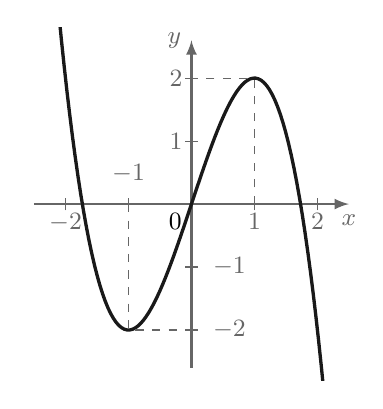
\begin{tikzpicture}[scale=0.8, >=latex]
    % 1. Giới hạn vùng hiển thị
    \clip (-2.6, -2.8) rectangle (2.6, 2.8);

    % 2. Trục tọa độ Oxy
    \draw[->, gray!80!black, thick] (-2.5, 0) -- (2.5, 0) node[below] {\small $x$};
    \draw[->, gray!80!black, thick] (0, -2.6) -- (0, 2.6) node[left] {\small $y$};
    \node[below left] at (0,0) {\small $0$};

    % 3. Đồ thị hàm số y = -x^3 + 3x
    \draw[very thick, gray!20!black, domain=-2.15:2.15, samples=100] 
        plot (\x, {-\x*\x*\x + 3*\x});

    % 4. Các đường dóng nét đứt
    \draw[dashed, gray!80!black] (-1, 0) -- (-1, -2) -- (0, -2);
    \draw[dashed, gray!80!black] (1, 0) -- (1, 2) -- (0, 2);

    % 5. Vạch chia và nhãn trên trục tọa độ
    % Trục Ox
    \draw[gray!80!black] (-2, -0.1) -- (-2, 0.1) node[below=2pt] {\small $-2$};
    \draw[gray!80!black] (-1, -0.1) -- (-1, 0.1) node[above=2pt] {\small $-1$};
    \draw[gray!80!black] (1, -0.1) -- (1, 0.1) node[below=2pt] {\small $1$};
    \draw[gray!80!black] (2, -0.1) -- (2, 0.1) node[below=2pt] {\small $2$};

    % Trục Oy
    \draw[gray!80!black] (-0.1, -2) -- (0.1, -2) node[right=2pt] {\small $-2$};
    \draw[gray!80!black] (-0.1, -1) -- (0.1, -1) node[right=2pt] {\small $-1$};
    \draw[gray!80!black] (-0.1, 1) -- (0.1, 1) node[left=2pt] {\small $1$};
    \draw[gray!80!black] (-0.1, 2) -- (0.1, 2) node[left=2pt] {\small $2$};
\end{tikzpicture}
\end{center}
}{
    \textbf{a)} & Trong bốn giá trị \( a, b, c, d \) có đúng một giá trị bằng 0.
    & \textcolor{amberorange}{$\bigcirc$} & \textcolor{amberorange}{$\bigcirc$} \\ \hline
    
    \textbf{b)} & Hàm số \( y = f(x) \) là hàm số lẻ trên tập \( \mathbb{R} \).
    & \textcolor{amberorange}{$\bigcirc$} & \textcolor{amberorange}{$\bigcirc$} \\ \hline
    
    \textbf{c)} & Điểm cực tiểu của đồ thị hàm số \( y = f(x) \) là \( x = -1 \).
    & \textcolor{amberorange}{$\bigcirc$} & \textcolor{amberorange}{$\bigcirc$} \\ \hline
    
    \textbf{d)} & Số nghiệm thực của phương trình \( f(x) = \dfrac{2025}{2026} \) là 3.
    & \textcolor{amberorange}{$\bigcirc$} & \textcolor{amberorange}{$\bigcirc$} \\
}

\questionTrueFalse{0}{6}{Cho hàm số \( y = f(x) = \dfrac{ax^2 + bx + c}{x + d} \) có bảng biến thiên như hình vẽ dưới đây.

\begin{center}

\begin{tikzpicture}
    \tkzTabInit[lgt=1.5, espcl=2.5]
    {$x$ /1, $y'$ /1, $y$ /2.5}
    {$-\infty$, $0$, $2$, $4$, $+\infty$}
    \tkzTabLine{, +, 0, -, d, +, 0, -, }
    \tkzTabVar{+/ $+\infty$ / , -/$2$, +D-/ $+\infty$ /  $-\infty$ / , +/ $-6$ / , -/ $-\infty$ /}
\end{tikzpicture}
\end{center}
}{
    \textbf{a)} & Hàm số \( y = f(x) \) đồng biến trên khoảng \( (0; 4) \).
    & \textcolor{amberorange}{$\bigcirc$} & \textcolor{amberorange}{$\bigcirc$} \\ \hline
    
    \textbf{b)} & Tích giá trị cực đại và cực tiểu của hàm số \( y = f(x) \) bằng \(-12\).
    & \textcolor{amberorange}{$\bigcirc$} & \textcolor{amberorange}{$\bigcirc$} \\ \hline
    
    \textbf{c)} & Cho điểm \( M \) có hoành độ lớn hơn 2, di chuyển trên đồ thị hàm số \( y = f(x) \). Giá trị nhỏ nhất của tổng khoảng cách từ điểm \( M \) đến hai trục tọa độ bằng \( 4 + 4\sqrt{2} \).
    & \textcolor{amberorange}{$\bigcirc$} & \textcolor{amberorange}{$\bigcirc$} \\ \hline
    
    \textbf{d)} & \( a + b + c + d = -5 \).
    & \textcolor{amberorange}{$\bigcirc$} & \textcolor{amberorange}{$\bigcirc$} \\
}

\questionTrueFalse{0}{7}{Cho hàm số \( y = x^3 - 3x^2 + 5 \) có đồ thị là \((C)\). Khi đó:}{
    \textbf{a)} & Hàm số đã cho nghịch biến trên khoảng \((0; 2)\).
    & \textcolor{amberorange}{$\bigcirc$} & \textcolor{amberorange}{$\bigcirc$} \\ \hline
    
    \textbf{b)} & Hàm số đã cho có hai điểm cực trị.
    & \textcolor{amberorange}{$\bigcirc$} & \textcolor{amberorange}{$\bigcirc$} \\ \hline
    
    \textbf{c)} & Giá trị nhỏ nhất của hàm số đã cho trên khoảng \((0; +\infty)\) bằng 2.
    & \textcolor{amberorange}{$\bigcirc$} & \textcolor{amberorange}{$\bigcirc$} \\ \hline
    
    \textbf{d)} & Tiếp tuyến của đồ thị \((C)\) tại điểm có hoành độ bằng 1 là đường thẳng có phương trình  
    \( y = -3x + 3 \).
    & \textcolor{amberorange}{$\bigcirc$} & \textcolor{amberorange}{$\bigcirc$} \\
}

\questionTrueFalse{0}{8}{Tại một khu bảo tồn thiên nhiên, các nhà khoa học đã thả một số cá thể của một loài động vật quý hiếm trong một khu rừng rộng 10 hecta và theo dõi sự tăng trưởng số lượng của chúng. Họ thấy rằng số lượng cá thể của loài động vật đó sau \( t \) năm kể từ khi nuôi tại khu bảo tồn được xấp xỉ bởi hàm số  
\(h(t) = 70 \log_2 \left( \dfrac{8t + 1}{t + 1} \right) + 30\)
(\( t \) là số thực dương) và tốc độ tăng trưởng số lượng cá thể của loài động vật đó tại thời điểm sau đúng \( t \) năm kể từ khi nuôi được xấp xỉ bởi hàm số  
\( h'(t) \)  
(đơn vị: cá thể /năm).}{
    \textbf{a)} & Thời điểm ban đầu, người ta thả nuôi 30 cá thể.
    & \textcolor{amberorange}{$\bigcirc$} & \textcolor{amberorange}{$\bigcirc$} \\ \hline
    
    \textbf{b)} & Sau 9 tháng kể từ khi bắt đầu nuôi, số lượng cá thể của loài động vật đó là 170.
    & \textcolor{amberorange}{$\bigcirc$} & \textcolor{amberorange}{$\bigcirc$} \\ \hline
    
    \textbf{c)} & Tốc độ tăng trưởng số lượng cá thể của loài động vật đó tại thời điểm đúng 6 năm kể từ khi nuôi là  
    \(\dfrac{10}{7}\) (cá thể /năm).
    & \textcolor{amberorange}{$\bigcirc$} & \textcolor{amberorange}{$\bigcirc$} \\ \hline
    
    \textbf{d)} & Số lượng cá thể của loài động vật đó không vượt quá 240.
    & \textcolor{amberorange}{$\bigcirc$} & \textcolor{amberorange}{$\bigcirc$} \\
}

\questionTrueFalse{0}{9}{Xét chuyển động của một tàu lượn trên đoạn đường ray có hình dạng một phần đồ thị của hàm số \( y = f(x) = \dfrac{135x - x^2 - x^3}{200} \) (\( x \geq 0 \)), trong đó \( x \) là khoảng cách theo phương ngang kể từ điểm \( A \), \( y \) là độ cao tương ứng của tàu lượn so với phương ngang \( AB \).  
Chọn hệ trục tọa độ \( Oxy \) như hình vẽ (đơn vị trên mỗi trục là 10m). Các kết quả được làm tròn đến hàng đơn vị.

\begin{center}
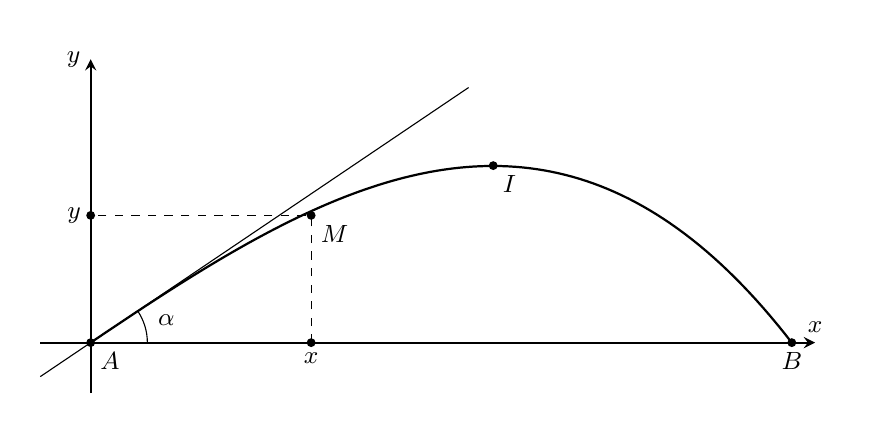
\begin{tikzpicture}[scale=0.8, >=latex]
    % 1. Giới hạn vùng hiển thị
    \clip (-1, -1) rectangle (12, 5);

    % 2. Các điểm tọa độ chính
    \coordinate (A) at (0, 0);
    \coordinate (B) at (11.13, 0);
    \coordinate (I) at (6.39, 2.81);
    \coordinate (M) at (3.5, 2.02);

    % 3. Trục tọa độ Oxy màu đen
    \draw[->, >=stealth, thick, black] (-0.8, 0) -- (11.5, 0) node[above] {\small $x$};
    \draw[->, >=stealth, thick, black] (0, -0.8) -- (0, 4.5) node[left] {\small $y$};

    % 4. Đồ thị chuyển động màu đen
    \draw[thick, black, domain=0:11.13, samples=100] 
        plot (\x, {(135*\x - \x*\x - \x*\x*\x)/200});

    % 5. Đường tiếp tuyến màu đen
    \draw[black, domain=-0.8:6] plot (\x, {0.675*\x});

    % 6. Đường dóng nét đứt màu đen
    \draw[dashed, black] (3.5, 0) -- (3.5, 2.02) -- (0, 2.02);

    % 7. Góc alpha tại gốc A
    \draw[black] (0.9, 0) arc (0:34:0.9);
    \node[black] at (1.2, 0.35) {\small $\alpha$};

    % 8. Các điểm nút màu đen và nhãn
    \fill[black] (A) circle (2pt) node[below right] {\small $A$};
    \fill[black] (B) circle (2pt) node[below] {\small $B$};
    \fill[black] (M) circle (2pt) node[below right] {\small $M$};
    \fill[black] (I) circle (2pt) node[below right] {\small $I$};
    \fill[black] (3.5, 0) circle (2pt) node[below] {\small $x$};
    \fill[black] (0, 2.02) circle (2pt) node[left] {\small $y$};
\end{tikzpicture}
\end{center}
}{
    \textbf{a)} & Độ dài đoạn \( AB \) bằng 11m.
    & \textcolor{amberorange}{$\bigcirc$} & \textcolor{amberorange}{$\bigcirc$} \\ \hline
    
    \textbf{b)} & Hàm số \( y = f(x) \) đạt cực trị tại \( x_0 = \dfrac{\sqrt{406} - 1}{3} \).
    & \textcolor{amberorange}{$\bigcirc$} & \textcolor{amberorange}{$\bigcirc$} \\ \hline
    
    \textbf{c)} & Độ cao lớn nhất của tàu lượn so với phương ngang \( AB \) là \( 64m \).
    & \textcolor{amberorange}{$\bigcirc$} & \textcolor{amberorange}{$\bigcirc$} \\ \hline
    
    \textbf{d)} & Khi tàu lượn đi qua điểm \( A \), tiếp tuyến của quỹ đạo tại \( A \) hợp với phương ngang \( AB \) một góc \( \alpha \approx 34^\circ \).
    & \textcolor{amberorange}{$\bigcirc$} & \textcolor{amberorange}{$\bigcirc$} \\
}

\questionTrueFalse{0}{10}{Cho hàm số \( y = f(x) = \dfrac{2x^2 - 5x + 9}{x - 5} \). Các mệnh đề sau đúng hay sai?}{
    \textbf{a)} & Đồ thị hàm số cắt trục tung tại điểm có tung độ bằng \(-\dfrac{9}{5}\).
    & \textcolor{amberorange}{$\bigcirc$} & \textcolor{amberorange}{$\bigcirc$} \\ \hline
    
    \textbf{b)} & Hàm số nghịch biến trên khoảng \((1; 9)\).
    & \textcolor{amberorange}{$\bigcirc$} & \textcolor{amberorange}{$\bigcirc$} \\ \hline
    
    \textbf{c)} & Có đúng một điểm trên đồ thị hàm số cách đều hai trục tọa độ.
    & \textcolor{amberorange}{$\bigcirc$} & \textcolor{amberorange}{$\bigcirc$} \\ \hline
    
    \textbf{d)} & Đồ thị hàm số có đường tiệm cận đứng là \(y = 5\).
    & \textcolor{amberorange}{$\bigcirc$} & \textcolor{amberorange}{$\bigcirc$} \\
}

\questionTrueFalse{0}{11}{Cho hàm số \( f(x) = \dfrac{3x + 1}{x + 4} \).}{
    \textbf{a)} & Hàm số \( f(x) \) có đạo hàm là \( f'(x) = \dfrac{11}{(x + 4)^2} \).
    & \textcolor{amberorange}{$\bigcirc$} & \textcolor{amberorange}{$\bigcirc$} \\ \hline
    
    \textbf{b)} & Với \( x_1, x_2 \in \mathbb{R} \) thỏa mãn \( x_1 < -4 < x_2 \) thì \( f(x_1) < f(x_2) \).
    & \textcolor{amberorange}{$\bigcirc$} & \textcolor{amberorange}{$\bigcirc$} \\ \hline
    
    \textbf{c)} & Tọa độ giao điểm của hai đường tiệm cận của đồ thị hàm số là: \((3; -4)\).
    & \textcolor{amberorange}{$\bigcirc$} & \textcolor{amberorange}{$\bigcirc$} \\ \hline
    
    \textbf{d)} & Giá trị nhỏ nhất của hàm số \( f(x) \) trên đoạn \([0; 1]\) bằng \(\dfrac{1}{4}\).
    & \textcolor{amberorange}{$\bigcirc$} & \textcolor{amberorange}{$\bigcirc$} \\
}

\questionTrueFalse{0}{12}{Cho hàm số \( y = \dfrac{2x-1}{x+1} \) có đồ thị \( (C) \).}{
    \textbf{a)} & Hàm số đồng biến trên tập xác định.
    & \textcolor{amberorange}{$\bigcirc$} & \textcolor{amberorange}{$\bigcirc$} \\ \hline
    
    \textbf{b)} & Đồ thị hàm số \( (C) \) có tâm đối xứng là điểm \( I(-1; 2) \).
    & \textcolor{amberorange}{$\bigcirc$} & \textcolor{amberorange}{$\bigcirc$} \\ \hline
    
    \textbf{c)} & Tiếp tuyến của đồ thị hàm số \( (C) \) tại giao điểm của đồ thị hàm số \( (C) \) với trục tung có phương trình là \( y = 3x - 1 \).
    & \textcolor{amberorange}{$\bigcirc$} & \textcolor{amberorange}{$\bigcirc$} \\ \hline
    
    \textbf{d)} & Số điểm thuộc đồ thị hàm số có tọa độ nguyên là 2.
    & \textcolor{amberorange}{$\bigcirc$} & \textcolor{amberorange}{$\bigcirc$} \\
}

\questionTrueFalse{0}{13}{Bác Bình dự định làm một bể cá bằng kính cường lực dạng hình hộp chữ nhật không nắp. Bể có thể tích \( 3m^3 \) và có chiều dài gấp đôi chiều rộng. Chi phí làm bể gồm hai phần: phần làm đáy bể là 500 ngàn đồng trên 1 m\(^2\) và phần làm mặt xung quanh là 400 ngàn đồng trên 1 m\(^2\). Chi phí vận hành bể cá trong một tháng là 400 ngàn đồng.

\begin{center}
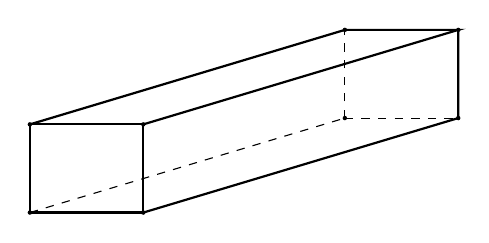
\begin{tikzpicture}[scale=0.8, >=latex]
    % 1. Định nghĩa tọa độ các đỉnh của hình hộp chữ nhật
    % Mặt trước
    \coordinate (A) at (0, 0);
    \coordinate (B) at (1.8, 0);
    \coordinate (C) at (1.8, 1.4);
    \coordinate (D) at (0, 1.4);
    
    % Mặt sau (đẩy sang phải và lên trên theo góc nhìn)
    \coordinate (A1) at (5, 1.5);
    \coordinate (B1) at (6.8, 1.5);
    \coordinate (C1) at (6.8, 2.9);
    \coordinate (D1) at (5, 2.9);

    % 2. Vẽ các cạnh nhìn thấy (Nét liền màu đen)
    % Khung mặt trước
    \draw[thick, black] (A) -- (B) -- (C) -- (D) -- cycle;
    % Các cạnh bên trên và bên phải
    \draw[thick, black] (D) -- (D1) -- (C1) -- (C);
    \draw[thick, black] (B) -- (B1) -- (C1);

    % 3. Vẽ các cạnh khuất bên trong (Nét đứt màu đen)
    \draw[dashed, black] (A) -- (A1);
    \draw[dashed, black] (A1) -- (B1);
    \draw[dashed, black] (A1) -- (D1);

    % 4. Các điểm nút tròn màu đen tại các đỉnh
    \foreach \p in {A, B, C, D, A1, B1, C1, D1} {
        \fill[black] (\p) circle (1pt);
    }
\end{tikzpicture}
\end{center}
}{
    \textbf{a)} & Chi phí vận hành bể cá trong một năm là 4,8 triệu đồng.
    & \textcolor{amberorange}{$\bigcirc$} & \textcolor{amberorange}{$\bigcirc$} \\ \hline
    
    \textbf{b)} & Nếu chiều rộng của bể là 1m thì chiều cao của bể là 3m.
    & \textcolor{amberorange}{$\bigcirc$} & \textcolor{amberorange}{$\bigcirc$} \\ \hline
    
    \textbf{c)} & Nếu chiều rộng của bể là \( x(m) \) thì diện tích xung quanh của bể là 
    \(\dfrac{9}{x}(m^2)\).
    & \textcolor{amberorange}{$\bigcirc$} & \textcolor{amberorange}{$\bigcirc$} \\ \hline
    
    \textbf{d)} & Chi phí ít nhất để làm bể 4,44 triệu đồng (làm tròn đến hàng phần trăm).
    & \textcolor{amberorange}{$\bigcirc$} & \textcolor{amberorange}{$\bigcirc$} \\
}

\questionTrueFalse{0}{14}{Cho hàm số \( f(x) = \dfrac{ax + b}{x + c} \) có giá trị lớn nhất trên đoạn \([3; 4]\) bằng 7 và có đồ thị \( y = f'(x) \) như hình vẽ.

\begin{center}
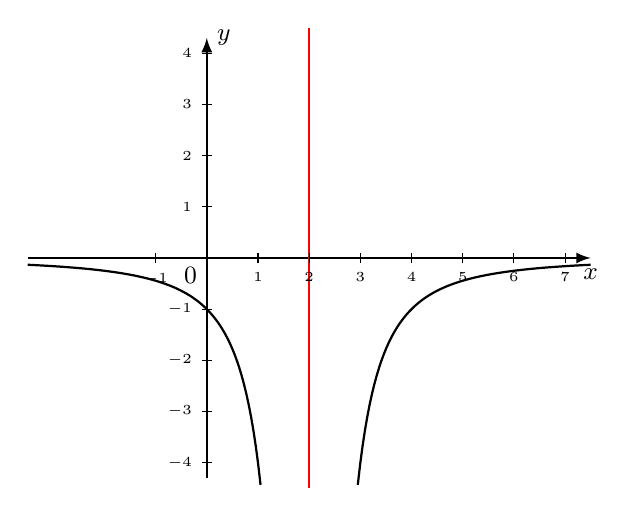
\begin{tikzpicture}[scale=0.65, >=latex]
    % 1. Giới hạn vùng hiển thị
    \clip (-3.5, -4.5) rectangle (7.8, 4.5);

    % 2. Trục tọa độ Oxy màu đen
    \draw[->, thick, black] (-3.5, 0) -- (7.5, 0) node[below] {\small $x$};
    \draw[->, thick, black] (0, -4.3) -- (0, 4.3) node[right] {\small $y$};
    \node[below left] at (0,0) {\small $0$};

    % 3. Đường tiệm cận đứng x = 2 màu đỏ
    \draw[thick, red] (2, -4.5) -- (2, 4.5);

    % 4. Đồ thị hàm số đạo hàm y = -4 / (x - 2)^2 (màu đen)
    % Nhánh bên trái (x < 2)
    \draw[thick, black, domain=-3.5:1.05, samples=100] 
        plot (\x, {-4/((\x - 2)*(\x - 2))});
    % Nhánh bên phải (x > 2)
    \draw[thick, black, domain=2.95:7.5, samples=100] 
        plot (\x, {-4/((\x - 2)*(\x - 2))});

    % 5. Vạch chia và nhãn trên trục Ox
    \foreach \x in {-1, 1, 2, 3, 4, 5, 6, 7} {
        \draw[black] (\x, -0.1) -- (\x, 0.1);
        \node[below, font=\tiny] at (\x, -0.1) {$\x$};
    }

    % 6. Vạch chia và nhãn trên trục Oy
    \foreach \y in {-4, -3, -2, -1, 1, 2, 3, 4} {
        \draw[black] (-0.1, \y) -- (0.1, \y);
        \node[left, font=\tiny] at (-0.1, \y) {$\y$};
    }
\end{tikzpicture}
\end{center}
}{
    \textbf{a)} & Đồ thị \( y = f'(x) \) có đường tiệm cận đứng là \( x = 2 \).
    & \textcolor{amberorange}{$\bigcirc$} & \textcolor{amberorange}{$\bigcirc$} \\ \hline
    
    \textbf{b)} & Hàm số \( f(x) \) nghịch biến trên khoảng \( (2; +\infty) \).
    & \textcolor{amberorange}{$\bigcirc$} & \textcolor{amberorange}{$\bigcirc$} \\ \hline
    
    \textbf{c)} & \( 3b + 2c = -2 \).
    & \textcolor{amberorange}{$\bigcirc$} & \textcolor{amberorange}{$\bigcirc$} \\ \hline
    
    \textbf{d)} & Giá trị nhỏ nhất của hàm số \( f(x) \) trên đoạn \([3; 4]\) bằng 6.
    & \textcolor{amberorange}{$\bigcirc$} & \textcolor{amberorange}{$\bigcirc$} \\
}


\questionTrueFalse{0}{15}{Cho hàm số \( y = \dfrac{-x^2 + 5x - 7}{x - 2} \), có đồ thị \( (C) \).}{
    \textbf{a)} & Hàm số nghịch biến trên \((-\infty; 1)\).
    & \textcolor{amberorange}{$\bigcirc$} & \textcolor{amberorange}{$\bigcirc$} \\ \hline
    
    \textbf{b)} & Khoảng cách giữa hai điểm cực trị của đồ thị \( (C) \) bằng \( 2\sqrt{5} \).
    & \textcolor{amberorange}{$\bigcirc$} & \textcolor{amberorange}{$\bigcirc$} \\ \hline
    
    \textbf{c)} & Đồ thị hàm số có tiệm cận xiên là đường thẳng \( y = -x - 3 \).
    & \textcolor{amberorange}{$\bigcirc$} & \textcolor{amberorange}{$\bigcirc$} \\ \hline
    
    \textbf{d)} & Giá trị nhỏ nhất của hàm số trên đoạn \([-2026; \dfrac{3}{2}]\) bằng 3.
    & \textcolor{amberorange}{$\bigcirc$} & \textcolor{amberorange}{$\bigcirc$} \\
}

\questionTrueFalse{0}{16}{Một hãng công nghệ dự định tung ra thị trường một loại tai nghe không dây mới. Chi phí sản xuất mỗi chiếc tai nghe là 500 nghìn đồng với giá bán ra niêm yết là 1,2 triệu đồng. Bộ phận bán hàng ước tính rằng, số lượng tai nghe bán ra được \( n(x) \) phụ thuộc vào chi phí quảng cáo \( x \) (đơn vị: triệu đồng) theo công thức \( n(x) = A + 30\ln(1+x) \). Biết rằng nếu chiếc tai nghe đóng cửa sổ thì bán được 190 sản phẩm.}{
    \textbf{a)} & \( A = 100 \).
    & \textcolor{amberorange}{$\bigcirc$} & \textcolor{amberorange}{$\bigcirc$} \\ \hline
    
    \textbf{b)} & Hàm lợi nhuận của hãng (tính theo triệu đồng) là \( L(x) = 70 + 21\ln(1+x) - 2x \).
    & \textcolor{amberorange}{$\bigcirc$} & \textcolor{amberorange}{$\bigcirc$} \\ \hline
    
    \textbf{c)} & Khi chi phí quảng cáo đang ở mức 6 triệu đồng thì lợi nhuận đạt 99 triệu đồng (kết quả làm tròn đến hàng đơn vị).
    & \textcolor{amberorange}{$\bigcirc$} & \textcolor{amberorange}{$\bigcirc$} \\ \hline
    
    \textbf{d)} & Để đạt lợi nhuận lớn nhất thì số tiền chi cho quảng cáo là 19,766 triệu đồng (kết quả làm tròn đến hàng phần nghìn).
    & \textcolor{amberorange}{$\bigcirc$} & \textcolor{amberorange}{$\bigcirc$} \\
}

\questionTrueFalse{0}{17}{Một công ty sau khi ra mắt sản phẩm mới đã ghi nhận lợi nhuận \( P(t) \) (đơn vị: triệu đồng) sau \( t \) tháng kinh doanh. Trong năm đầu tiên, giá sử mối liên hệ giữa lợi nhuận và thời gian kinh doanh được mô hình hóa bởi hàm số:
\(P(t) = -t^3 + 10t^2 + 63t - 45, \, 0 \leq t \leq 12.\)}{
    \textbf{a)} & Lợi nhuận của công ty sau 1 quý là 27 triệu đồng.
    & \textcolor{amberorange}{$\bigcirc$} & \textcolor{amberorange}{$\bigcirc$} \\ \hline
    
    \textbf{b)} & Lợi nhuận của công ty đạt mức tối đa tại thời điểm \( t = 9 \).
    & \textcolor{amberorange}{$\bigcirc$} & \textcolor{amberorange}{$\bigcirc$} \\ \hline
    
    \textbf{c)} & Tại thời điểm \( t = 4 \) thì tốc độ tăng trưởng lợi nhuận là lớn nhất.
    & \textcolor{amberorange}{$\bigcirc$} & \textcolor{amberorange}{$\bigcirc$} \\ \hline
    
    \textbf{d)} & Hàm số biểu thị tốc độ tăng trưởng lợi nhuận \( P'(t) = -3t^2 + 20t + 63t \).
    & \textcolor{amberorange}{$\bigcirc$} & \textcolor{amberorange}{$\bigcirc$} \\
}


\questionTrueFalse{0}{18}{Cho hàm số \( y = f(x) = x + \dfrac{1}{x-1} \).}{
    \textbf{a)} & \( f'(x) = 1 - \dfrac{1}{(x-1)^2} \).
    & \textcolor{amberorange}{$\bigcirc$} & \textcolor{amberorange}{$\bigcirc$} \\ \hline
    
    \textbf{b)} & Phương trình \( f'(x) = 0 \) có hai nghiệm phân biệt \( x = 0 \) và \( x = 2 \).
    & \textcolor{amberorange}{$\bigcirc$} & \textcolor{amberorange}{$\bigcirc$} \\ \hline
    
    \textbf{c)} & Hàm số đã cho có bảng biến thiên như sau:
    
    \begin{center}
    
\begin{tikzpicture}
        \tkzTabInit[lgt=1, espcl=2]
        {$x$ /0.6, $y'$ /0.6, $y$ /1.5}
        {$-\infty$, $0$, $1$, $2$, $+\infty$}
        \tkzTabLine{, +, 0, -, d, -, 0, +, }
        \tkzTabVar{-/ $-\infty$ / , +/ $-1$ / , -D+/ $-\infty$ / / $+\infty$ / , -/$3$, +/ $+\infty$ /}
    \end{tikzpicture}
    \end{center}
    & \textcolor{amberorange}{$\bigcirc$} & \textcolor{amberorange}{$\bigcirc$} \\ \hline
    
    \textbf{d)} & Hàm số đã cho có đồ thị như sau:
    
    \begin{center}
    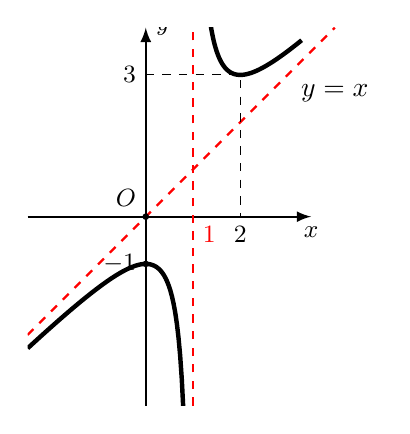
\begin{tikzpicture}[>=latex, scale=0.6]
        \clip (-2.5, -4) rectangle (5, 4);
        % 1. Vẽ hệ trục tọa độ
        \draw[->, black, thick] (-2.5, 0) -- (3.5, 0) node[below] {\small $x$};
        \draw[->, black, thick] (0, -4) -- (0, 4) node[right] {\small $y$};
        
        
        % 2. Vẽ tiệm cận đứng x = 1
        \draw[dashed, red, thick] (1,-4) -- (1,4);
        \node[below right, red] at (1,0) {\small $1$};
        
        % 3. Vẽ tiệm cận xiên y = x
        \draw[dashed, red, thick] (-3,-3) -- (4,4);
        \node[below] at (4,3) {$y = x$};
        
        % 4. Vẽ đồ thị hàm số y = x + 1/(x-1)
        \draw[ultra thick, samples=100, domain=-2.5:0.9] 
            plot (\x, {\x + 1/(\x - 1)});
        \draw[ultra thick, samples=100, domain=1.1:3.3] 
            plot (\x, {\x + 1/(\x - 1)});
        
        % 5. Đánh dấu các điểm cực trị
        \draw[dashed, black] (0,-1) -- (0,0);
        \node[left] at (0,-1) {\small $-1$};
        \fill (0,-1) circle (2pt);
        
        \draw[dashed, black] (0,3)--(2,3) -- (2,0);
        \node[below] at (2,0) {\small $2$};
        \node[left] at (0,3) {\small $3$};
        
        % Giao điểm với trục Oy
        \fill (0,0) circle (2pt);
        \node[above left] at (0,0) {\small $O$};
        
    \end{tikzpicture}
    \end{center}
    & \textcolor{amberorange}{$\bigcirc$} & \textcolor{amberorange}{$\bigcirc$} \\
}

\questionTrueFalse{0}{19}{Trang trại nhà ông A chuyên sản xuất các loại thực phẩm cho nhà hàng của ông B. Hai ông thỏa thuận rằng, hàng ngày ông A cung cấp cho ông B số lượng thực phẩm theo đơn đặt hàng của ông B (tối đa 100 kg thực phẩm). Nếu số lượng đặt hàng là \( x \) kg thực phẩm thì giá bán cho mỗi kg được biểu diễn bởi công thức \( P(x) = 30 - \dfrac{1}{1000}x^2 \) (ngàn đồng). Chi phí để ông A sản xuất \( x \) kg sản phẩm là \( C(x) = 200 + 15x \) (ngàn đồng). Khi đó}{
    \textbf{a)} & Chi phí sản xuất \( 100kg \) thực phẩm là \( 350 \) ngàn đồng.
    & \textcolor{amberorange}{$\bigcirc$} & \textcolor{amberorange}{$\bigcirc$} \\ \hline
    
    \textbf{b)} & Số tiền thu được khi bán \( 100kg \) thực phẩm cho nhà hàng ông B là \( 200 \) ngàn đồng.
    & \textcolor{amberorange}{$\bigcirc$} & \textcolor{amberorange}{$\bigcirc$} \\ \hline
    
    \textbf{c)} & Lợi nhuận ông A thu được khi bán \( xkg, x \in (0;100) \) thực phẩm cho ông B là \( L(x) = x \cdot P(x) - C(x) \).
    & \textcolor{amberorange}{$\bigcirc$} & \textcolor{amberorange}{$\bigcirc$} \\ \hline
    
    \textbf{d)} & Lợi nhuận lớn nhất mà ông A có được trong một ngày là \( 507 \) ngàn đồng (làm tròn đến hàng đơn vị).
    & \textcolor{amberorange}{$\bigcirc$} & \textcolor{amberorange}{$\bigcirc$} \\
}

\questionTrueFalse{0}{20}{Cho hàm số  
\(y = f(x) = \dfrac{ax + b}{cx - 1} \quad (\text{với } a, b, c \text{ là các số thực}) \text{ có đồ thị được cho ở hình} \)

\begin{center}
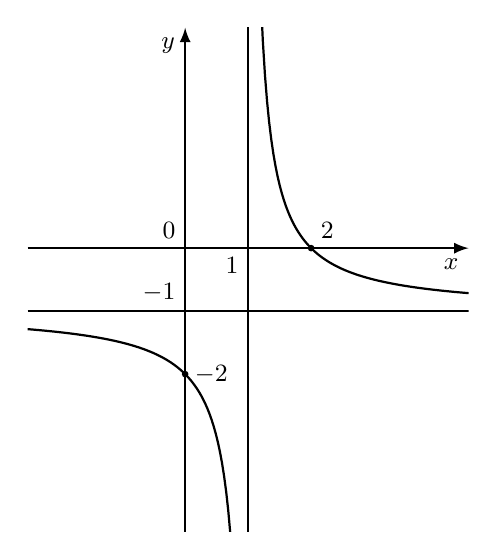
\begin{tikzpicture}[scale=0.8, >=latex]
    % 1. Giới hạn vùng hiển thị
    \clip (-2.5, -4.5) rectangle (4.5, 3.5);

    % 2. Trục tọa độ Oxy màu đen
    \draw[->, thick, black] (-2.5, 0) -- (4.5, 0) node[below left] {\small $x$};
    \draw[->, thick, black] (0, -4.5) -- (0, 3.5) node[below left] {\small $y$};
    \node[above left] at (0,0) {\small $0$};

    % 3. Các đường tiệm cận (nét liền màu đen)
    \draw[thick, black] (1, -4.5) -- (1, 3.8); % Tiệm cận đứng x = 1
    \draw[thick, black] (-2.5, -1) -- (4.5, -1); % Tiệm cận ngang y = -1

    % 4. Đồ thị hàm số y = (-x + 2)/(x - 1)
    % Nhánh trái (x < 1)
    \draw[thick, black, domain=-2.5:0.75, samples=100] 
        plot (\x, {(-\x + 2)/(\x - 1)});
    % Nhánh phải (x > 1)
    \draw[thick, black, domain=1.2:4.5, samples=100] 
        plot (\x, {(-\x + 2)/(\x - 1)});

    % 5. Đánh dấu các nhãn số và điểm cắt
    % Giá trị 1 trên trục Ox
    \node[below left] at (1, 0) {\small $1$};
    
    % Giá trị 2 trên trục Ox
    \fill[black] (2, 0) circle (1.5pt);
    \node[above right] at (2, 0) {\small $2$};

    % Giá trị -1 trên trục Oy
    \node[above left] at (0, -1) {\small $-1$};

    % Giá trị -2 trên trục Oy
    \fill[black] (0, -2) circle (1.5pt);
    \node[right] at (0, -2) {\small $-2$};
\end{tikzpicture}
\end{center}
}{
    \textbf{a)} & Đồ thị hàm số có một đường tiệm cận đứng \( x = 1 \) và một đường tiệm cận ngang \( y = -1 \).
    & \textcolor{amberorange}{$\bigcirc$} & \textcolor{amberorange}{$\bigcirc$} \\ \hline
    
    \textbf{b)} & Giá trị \( a + 2b - 3c = 5 \).
    & \textcolor{amberorange}{$\bigcirc$} & \textcolor{amberorange}{$\bigcirc$} \\ \hline
    
    \textbf{c)} & Đạo hàm \( f'(x) < 0 \) với mọi \( x \in \mathbb{R} \setminus \{1\} \).
    & \textcolor{amberorange}{$\bigcirc$} & \textcolor{amberorange}{$\bigcirc$} \\ \hline
    
    \textbf{d)} & M, N là hai điểm thuộc hai nhánh khác nhau của đồ thị khi đó MN ngắn nhất bằng \( \sqrt{10} \).
    & \textcolor{amberorange}{$\bigcirc$} & \textcolor{amberorange}{$\bigcirc$} \\
}

\questionTrueFalse{0}{21}{Cho hàm số  
\( y = f(x) = ax^3 + bx^2 + cx + d \)
có bảng biến thiên được cho như bảng sau

\begin{center}

\begin{tikzpicture}
    % Khởi tạo bảng biến thiên
    \tkzTabInit[lgt=1.5, espcl=2.5, deltacl=0.6]
        {$x$ / 0.8, $f'(x)$ / 0.8, $f(x)$ / 1.8}
        {$-\infty$, $0$, $3$, $+\infty$}
    
    % Dòng dấu của f'(x)
    \tkzTabLine{, +, 0, -, 0, +, }
    
    % Dòng chiều biến thiên của f(x)
    \tkzTabVar{-/ $-\infty$, +/ $2$, -/ $-4$, +/ $+\infty$}
\end{tikzpicture}
\end{center}
}{
    \textbf{a)} & \( f(2025) > f(2026) \).
    & \textcolor{amberorange}{$\bigcirc$} & \textcolor{amberorange}{$\bigcirc$} \\ \hline
    
    \textbf{b)} & Hàm số đạt cực đại tại \( x = 3 \).
    & \textcolor{amberorange}{$\bigcirc$} & \textcolor{amberorange}{$\bigcirc$} \\ \hline
    
    \textbf{c)} & Giá trị lớn nhất của hàm số trên \((-\infty; 3]\) bằng 0.
    & \textcolor{amberorange}{$\bigcirc$} & \textcolor{amberorange}{$\bigcirc$} \\ \hline
    
    \textbf{d)} & Trong bốn hệ số \( a, b, c, d \) chỉ có hệ số \( b \) nhận giá trị âm.
    & \textcolor{amberorange}{$\bigcirc$} & \textcolor{amberorange}{$\bigcirc$} \\
}


\questionTrueFalse{0}{22}{Cho hàm số \( f(x) = \dfrac{x - 2}{x - 1} \) có đồ thị là đường cong \( (C) \).}{
    \textbf{a)} & Hàm số đồng biến trên khoảng \((-\infty; +\infty)\).
    & \textcolor{amberorange}{$\bigcirc$} & \textcolor{amberorange}{$\bigcirc$} \\ \hline
    
    \textbf{b)} & Đồ thị \( (C) \) như hình vẽ dưới đây.
    
   \begin{center}
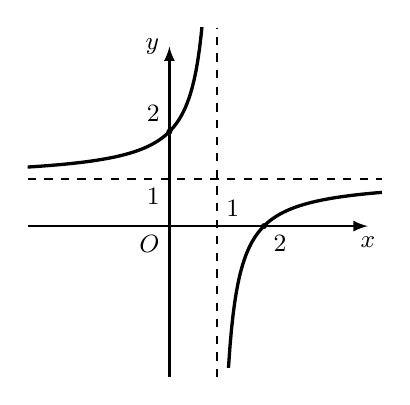
\begin{tikzpicture}[scale=0.6, >=latex]
    % 1. Giới hạn vùng hiển thị
    \clip (-3, -3.2) rectangle (4.5, 4.2);

    % 2. Trục tọa độ Oxy (màu đen)
    \draw[->, thick, black] (-3, 0) -- (4.2, 0) node[below] {\small $x$};
    \draw[->, thick, black] (0, -3.2) -- (0, 3.8) node[left] {\small $y$};
    \node[below left] at (0,0) {\small $O$};

    % 3. Đường tiệm cận đứng x = 1 và tiệm cận ngang y = 1 (nét đứt màu đen)
    \draw[dashed, thick, black] (1, -3.2) -- (1, 4.2);
    \draw[dashed, thick, black] (-3, 1) -- (4.5, 1);

    % 4. Đồ thị hàm số y = (x - 2)/(x - 1) (màu đen)
    % Nhánh trái (x < 1)
    \draw[very thick, black, domain=-3:0.75, samples=100] 
        plot (\x, {(\x - 2)/(\x - 1)});
    % Nhánh phải (x > 1)
    \draw[very thick, black, domain=1.25:4.5, samples=100] 
        plot (\x, {(\x - 2)/(\x - 1)});

    % 5. Đánh dấu các số và điểm giao trên các trục
    % Trên trục Ox
    \node[above right] at (1, 0) {\small $1$};
    \fill[black] (2, 0) circle (1.8pt);
    \node[below right] at (2, 0) {\small $2$};

    % Trên trục Oy
    \node[below left] at (0, 1) {\small $1$};
    \fill[black] (0, 2) circle (1.8pt);
    \node[above left] at (0, 2) {\small $2$};
\end{tikzpicture}
\end{center}
    & \textcolor{amberorange}{$\bigcirc$} & \textcolor{amberorange}{$\bigcirc$} \\ \hline
    
    \textbf{c)} & Gọi \( M, m \) lần lượt là giá trị lớn nhất, giá trị nhỏ nhất của hàm số \( y = |f(x)| \) trên đoạn \(\left[\dfrac{3}{2}; 3\right]\). Khi đó:  
    \( 2M + 2026m = 2027 \).
    & \textcolor{amberorange}{$\bigcirc$} & \textcolor{amberorange}{$\bigcirc$} \\ \hline
    
    \textbf{d)} & Đồ thị \( (C) \) có đường tiệm cận ngang \( y = 1 \) và đường tiệm cận đứng \( x = 1 \).
    & \textcolor{amberorange}{$\bigcirc$} & \textcolor{amberorange}{$\bigcirc$} \\
}

\questionTrueFalse{0}{23}{Cho hàm số \( y = f(x) \) có bảng biến thiên như sau.

\begin{center}

\begin{tikzpicture}
    \tkzTabInit[lgt=1.5, espcl=2.5]
    {$x$ /1, $f'(x)$ /1}
    {$-\infty$, $-1$, $1$, $2$, $+\infty$}
    \tkzTabLine{, +, 0, -, 0, +, 0, +, }
\end{tikzpicture}
\end{center}
}{
    \textbf{a)} & Hàm số đồng biến trên khoảng \((-\infty; -2)\).
    & \textcolor{amberorange}{$\bigcirc$} & \textcolor{amberorange}{$\bigcirc$} \\ \hline
    
    \textbf{b)} & Biết rằng hàm số \(y = f(x)\) có đồ thị đi qua điểm \(A(1;3)\) và đạt giá trị nhỏ nhất trên đoạn \([-1; 2]\) tại \(x = 1\). Khi đó:  
    \(f(-1) + f(2) - 2f(1) > 0\).
    & \textcolor{amberorange}{$\bigcirc$} & \textcolor{amberorange}{$\bigcirc$} \\ \hline
    
    \textbf{c)} & Hàm số \(y = f(x)\) có 2 điểm cực tiểu.
    & \textcolor{amberorange}{$\bigcirc$} & \textcolor{amberorange}{$\bigcirc$} \\ \hline
    
    \textbf{d)} & Hàm số đạt cực đại tại \(x = 2\).
    & \textcolor{amberorange}{$\bigcirc$} & \textcolor{amberorange}{$\bigcirc$} \\
}

\questionTrueFalse{0}{24}{Sau khi phát hiện một bệnh dịch, các chuyên gia y tế ước tính số người nhiễm bệnh kể từ ngày xuất hiện bệnh nhân đầu tiên đến ngày thứ \( t \) là 
\( f(t) = 45t^2 - t^3 \) với \( t \geq 0 \). Nếu coi \( y = f(t) \) là hàm số xác định trên \([0; +\infty)\) thì \( f'(t) \) được xem là tốc độ truyền bệnh (người/ngày) tại thời điểm \( t \).}{
    \textbf{a)} & Đến ngày thứ 45 thì không còn người nhiễm bệnh.
    & \textcolor{amberorange}{$\bigcirc$} & \textcolor{amberorange}{$\bigcirc$} \\ \hline
    
    \textbf{b)} & Trong 35 ngày đầu tiên thì số người nhiễm bệnh luôn tăng.
    & \textcolor{amberorange}{$\bigcirc$} & \textcolor{amberorange}{$\bigcirc$} \\ \hline
    
    \textbf{c)} & Tốc độ truyền bệnh tại thời điểm \( t \) là \( f'(t) = 90t - 3t^2 \).
    & \textcolor{amberorange}{$\bigcirc$} & \textcolor{amberorange}{$\bigcirc$} \\ \hline
    
    \textbf{d)} & Số người bị nhiễm bệnh từ ngày xuất hiện bệnh nhân đầu tiên đến ngày thứ 13 là 4752.
    & \textcolor{amberorange}{$\bigcirc$} & \textcolor{amberorange}{$\bigcirc$} \\
}


\questionTrueFalse{0}{25}{Đồ thị \( C \) của hàm số \( y = f(x) = \dfrac{ax + 8}{x + b} \) có bảng biến thiên như hình bên.

\begin{center}

\begin{tikzpicture}
    \tkzTabInit[lgt=1.5, espcl=2.5]
    {$x$ /1, $y'$ /1, $y$ /2.5}
    {$-\infty$, $-2$, $+\infty$}
    \tkzTabLine{, -, d, -, }
    \tkzTabVar{+/ $3$ / , -D+/ $-\infty$ / $+\infty$ / , -/ $3$ /}
\end{tikzpicture}
\end{center}
}{
    \textbf{a)} & Đồ thị hàm số \( y = f(x) \) có tâm đối xứng là \( I(3; -2) \).
    & \textcolor{amberorange}{$\bigcirc$} & \textcolor{amberorange}{$\bigcirc$} \\ \hline
    
    \textbf{b)} & Tập giá trị của hàm số \( y = f(x) \) là  
    \(T = \mathbb{R} \setminus \{3\}\).
    & \textcolor{amberorange}{$\bigcirc$} & \textcolor{amberorange}{$\bigcirc$} \\ \hline
    
    \textbf{c)} & \( a + 2b = -1 \).
    & \textcolor{amberorange}{$\bigcirc$} & \textcolor{amberorange}{$\bigcirc$} \\ \hline
    
    \textbf{d)} & Xét điểm \( A \in C \), tổng khoảng cách từ \( A \) đến hai đường tiệm cận của \( C \) luôn lớn hơn 2,83.
    & \textcolor{amberorange}{$\bigcirc$} & \textcolor{amberorange}{$\bigcirc$} \\
}

\questionTrueFalse{0}{26}{Diện tích bao phủ của cỏ Posidonia (một loài tảo biển) trên đáy ở một vùng vịnh theo thời gian được một nhóm các nhà sinh vật học quan sát và mô hình hoá bởi hàm số  
\(f(t) = \dfrac{k}{1 + 14e^{-0,3t}}\) 
(hecta), trong đó thời gian \( t \) tính bằng năm, \( k \) là số thực dương. Năm 2024 (ứng với \( t = 0 \)) là thời điểm các nhà sinh vật học bắt đầu quan sát, lúc đó diện tích của cỏ Posidonia đã bao phủ là 1 (hecta).}{
    \textbf{a)} & Giá trị \( k = 2 \).
    & \textcolor{amberorange}{$\bigcirc$} & \textcolor{amberorange}{$\bigcirc$} \\ \hline
    
    \textbf{b)} & Theo thời gian, diện tích bao phủ của cỏ Posidonia ở vịnh này sẽ không vượt quá 15 (hecta).
    & \textcolor{amberorange}{$\bigcirc$} & \textcolor{amberorange}{$\bigcirc$} \\ \hline
    
    \textbf{c)} & Khi diện tích cỏ bao phủ 5 (hecta) thì tốc độ bao phủ ở thời điểm đó là 1 (hecta/năm).
    & \textcolor{amberorange}{$\bigcirc$} & \textcolor{amberorange}{$\bigcirc$} \\ \hline
    
    \textbf{d)} & Nhóm các nhà sinh vật học dự đoán được tốc độ thay đổi diện tích bao phủ của cỏ Posidonia trong năm 2035 là nhanh nhất.
    & \textcolor{amberorange}{$\bigcirc$} & \textcolor{amberorange}{$\bigcirc$} \\
}

\questionTrueFalse{0}{27}{Cho hàm số  
\(f(x) = 3x - \log_5(x - 1)\)}{
    \textbf{a)} & Đạo hàm của hàm số \( f'(x) \) là  
    \(f'(x) = 3 - \dfrac{1}{x - 1}, \quad \forall x \in (1; +\infty).\)
    & \textcolor{amberorange}{$\bigcirc$} & \textcolor{amberorange}{$\bigcirc$} \\ \hline
    
    \textbf{b)} & Hàm số \( f(x) \) có một điểm cực tiểu.
    & \textcolor{amberorange}{$\bigcirc$} & \textcolor{amberorange}{$\bigcirc$} \\ \hline
    
    \textbf{c)} & Hàm số đồng biến trên khoảng \((2; +\infty)\).
    & \textcolor{amberorange}{$\bigcirc$} & \textcolor{amberorange}{$\bigcirc$} \\ \hline
    
    \textbf{d)} & Giá trị nhỏ nhất của hàm số trên khoảng \((1; +\infty)\) lớn hơn  
    \(\dfrac{9}{2}\).
    & \textcolor{amberorange}{$\bigcirc$} & \textcolor{amberorange}{$\bigcirc$} \\
}


\questionTrueFalse{0}{28}{Một xưởng mộc dùng gỗ sỏi để sản xuất 5 chiếc bàn mỗi ngày. Chi phí cho mỗi lần vận chuyển nguyên liệu là 5625 USD, chi phí để lưu trữ một đơn vị nguyên liệu là 10 USD mỗi ngày, trong đó một đơn vị là lượng nguyên liệu cần thiết để sản xuất một chiếc bàn, và lưu ý rằng trong mỗi ngày của chu kì sản xuất (thời gian giữa hai lần nhập nguyên liệu liên tiếp) thì lượng nguyên liệu lưu trữ trung bình mỗi ngày được tính bằng một nửa tổng lượng nguyên liệu tồn kho đầu kì và lượng nguyên liệu tồn kho cuối kì. Giả sử nguyên liệu được nhập về sau mỗi \( x \) ngày.}{
    \textbf{a)} & Một chu kì sản xuất, xưởng mộc phải nhập về \( 5x \) đơn vị nguyên liệu.
    & \textcolor{amberorange}{$\bigcirc$} & \textcolor{amberorange}{$\bigcirc$} \\ \hline
    
    \textbf{b)} & Chi phí để lưu trữ nguyên liệu trong \( x \) ngày của một chu kì sản xuất là \( 50x^2 \) USD.
    & \textcolor{amberorange}{$\bigcirc$} & \textcolor{amberorange}{$\bigcirc$} \\ \hline
    
    \textbf{c)} & Hàm chi phí trung bình mỗi ngày trong một chu kì sản xuất là  
    \(c(x) = 50x + \dfrac{5625}{x}\).
    & \textcolor{amberorange}{$\bigcirc$} & \textcolor{amberorange}{$\bigcirc$} \\ \hline
    
    \textbf{d)} & Để chi phí trung bình mỗi ngày của một chu kì sản xuất là ít nhất thì xưởng mộc nên nhập hàng sau mỗi 15 ngày và mỗi lần nhập về 75 đơn vị nguyên liệu.
    & \textcolor{amberorange}{$\bigcirc$} & \textcolor{amberorange}{$\bigcirc$} \\
}

\questionTrueFalse{0}{29}{Cho hàm số \( y = f(x) = \dfrac{2x - 3}{x - 1} \) có đồ thị \((C)\).}{
    \textbf{a)} & Hàm số \( y = f(x) \) đồng biến trên mỗi khoảng \((-\infty; 1)\) và \((1; +\infty)\).
    & \textcolor{amberorange}{$\bigcirc$} & \textcolor{amberorange}{$\bigcirc$} \\ \hline
    
    \textbf{b)} & Hàm số \( y = f(x) \) không có cực trị.
    & \textcolor{amberorange}{$\bigcirc$} & \textcolor{amberorange}{$\bigcirc$} \\ \hline
    
    \textbf{c)} & Giá trị lớn nhất của hàm số \( f(x) \) trên đoạn \([-3; 0]\) là 3.
    & \textcolor{amberorange}{$\bigcirc$} & \textcolor{amberorange}{$\bigcirc$} \\ \hline
    
    \textbf{d)} & Tâm đối xứng của đồ thị \((C)\) có tọa độ là \((2; 1)\).
    & \textcolor{amberorange}{$\bigcirc$} & \textcolor{amberorange}{$\bigcirc$} \\
}

\questionTrueFalse{0}{30}{Một cửa hàng bán tạp chí với giá 20 nghìn đồng một cuốn.  
Chi phí xuất bản \( x \) cuốn tạp chí (bao gồm: lương cán bộ, công nhân viên, giấy in,..) được cho bởi công thức \( C(x) = 0,0001x^2 - 0,2x + 10000 \), \( C'(x) \) được tính theo đơn vị vạn đồng. Chi phí phát hành cho mỗi cuốn là 4 nghìn đồng. Các khoản thu bao gồm: tiền bán tạp chí và 90 triệu đồng trợ cấp cho báo chí. Giả sử số cuốn in ra đều được bán hết.  
Xét tính đúng sai của các mệnh đề sau:}{
    \textbf{a)} & Tổng chi phí \( T(x) \) (xuất bản và phát hành) cho \( x \) cuốn tạp chí là  
    \(T(x) = 0,0001x^2 + 0,2x + 10000\).
    & \textcolor{amberorange}{$\bigcirc$} & \textcolor{amberorange}{$\bigcirc$} \\ \hline
    
    \textbf{b)} & Số tiền lãi khi in \( x \) cuốn tạp chí là \( L(x) = 0,0001x^2 + 1,8x - 1000\).
    & \textcolor{amberorange}{$\bigcirc$} & \textcolor{amberorange}{$\bigcirc$} \\ \hline
    
    \textbf{c)} & Để có lãi cần in từ 574 đến 17426 cuốn.
    & \textcolor{amberorange}{$\bigcirc$} & \textcolor{amberorange}{$\bigcirc$} \\ \hline
    
    \textbf{d)} & Lãi nhiều nhất khi in 10000 cuốn.
    & \textcolor{amberorange}{$\bigcirc$} & \textcolor{amberorange}{$\bigcirc$} \\
}

\questionTrueFalse{0}{31}{Cho hàm số \( y = \dfrac{ax^2 + bx + c}{x + d} \) có đồ thị như hình vẽ dưới đây. Biết rằng điểm \( O(0;0) \) là điểm cực đại của đồ thị hàm số.

\begin{center}
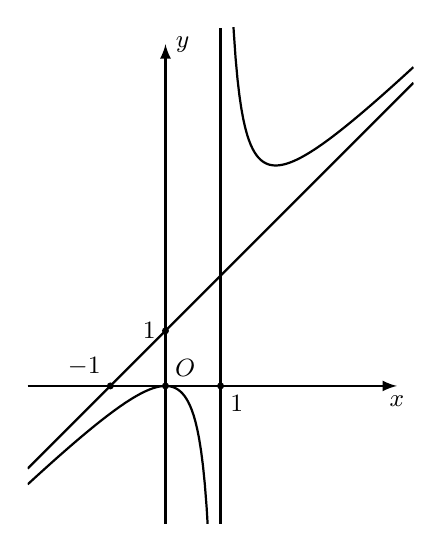
\begin{tikzpicture}[scale=0.7, >=latex]
    % 1. Giới hạn vùng hiển thị
    \clip (-2.5, -2.5) rectangle (4.5, 6.5);

    % 2. Trục tọa độ Oxy màu đen
    \draw[->, thick, black] (-2.5, 0) -- (4.2, 0) node[below] {\small $x$};
    \draw[->, thick, black] (0, -2.5) -- (0, 6.2) node[right] {\small $y$};
    \node[above right] at (0,0) {\small $O$};

    % 3. Tiệm cận đứng x = 1 (màu đen)
    \draw[thick, black] (1, -2.5) -- (1, 6.5);

    % 4. Tiệm cận xiên y = x + 1 (màu đen)
    \draw[thick, black, domain=-2.5:4.5] plot (\x, {\x + 1});

    % 5. Đồ thị hàm số y = x^2 / (x - 1) (màu đen)
    % Nhánh trái (x < 1)
    \draw[thick, black, domain=-2.5:0.85, samples=100] 
        plot (\x, {(\x*\x)/(\x - 1)});
    % Nhánh phải (x > 1)
    \draw[thick, black, domain=1.1:4.5, samples=100] 
        plot (\x, {(\x*\x)/(\x - 1)});

    % 6. Điểm đặc biệt và nhãn số
    % Điểm cực đại tại gốc tọa độ O(0,0)
    \fill[black] (0, 0) circle (1.8pt);

    % Giao điểm trên trục Ox: x = -1
    \fill[black] (-1, 0) circle (1.8pt);
    \node[above left] at (-1, 0) {\small $-1$};

    % Giao điểm tiệm cận xiên trên trục Oy: y = 1
    \fill[black] (0, 1) circle (1.8pt);
    \node[left] at (0, 1) {\small $1$};

    % Giao điểm tiệm cận đứng trên trục Ox: x = 1
    \fill[black] (1, 0) circle (1.8pt);
    \node[below right] at (1, 0) {\small $1$};
\end{tikzpicture}
\end{center}
}{
    \textbf{a)} & Phương trình đường tiệm cận xiên của đồ thị hàm số là  
    \( y = x + 1 \).
    & \textcolor{amberorange}{$\bigcirc$} & \textcolor{amberorange}{$\bigcirc$} \\ \hline
    
    \textbf{b)} & Điểm cực tiểu của đồ thị hàm số là \( T(2;4) \).
    & \textcolor{amberorange}{$\bigcirc$} & \textcolor{amberorange}{$\bigcirc$} \\ \hline
    
    \textbf{c)} & Hàm số đồng biến trên \( (1;+\infty) \).
    & \textcolor{amberorange}{$\bigcirc$} & \textcolor{amberorange}{$\bigcirc$} \\ \hline
    
    \textbf{d)} & Gọi \( A, B \) là hai điểm di động trên đồ thị hàm số sao cho các tiếp tuyến của đồ thị hàm số tại \( A \) và \( B \) luôn song song với nhau. Khi khoảng cách từ điểm \( M(4;1) \) đến đường thẳng \( AB \) lớn nhất thì độ dài đoạn thẳng \( AB \) bằng \( 2\sqrt{5} \).
    & \textcolor{amberorange}{$\bigcirc$} & \textcolor{amberorange}{$\bigcirc$} \\
}

\questionTrueFalse{0}{32}{Đậu đỏ là một loại thực phẩm quen thuộc trong bữa ăn của người Việt Nam. Ngoài giá trị dinh dưỡng cao, đậu đỏ còn có nhiều công dụng tuyệt vời cho sức khỏe và sắc đẹp như: Chống ôxy hóa, giúp cơ bắp con người khỏe mạnh, tăng cường sức khỏe cho tim mạch con người, lợi ích hệ tiêu hóa, bổ thận, cung cấp vitamin bổ dưỡng cho cơ thể, đào thải độc tố, giải độc, tốt cho hệ miễn dịch, giúp huyết áp ổn định, da đẹp. Cây đậu đỏ khi trồng có chiều cao 6 cm. Khảo sát cho thấy độ cao tính bằng centimet của cây đậu đỏ tại thời điểm \( t \) kể từ khi được trồng được cho bởi hàm số \( h(t) = -0,005t^4 + bt^3 + c \) (Trong đó \( b, c \in \mathbb{R} \)), với \( t \) tính theo tuần. Giả sử \( h'(t) \) là tốc độ tăng chiều cao của cây đậu đỏ sau khi trồng. (Đơn vị của \( t \) là giờ.) \( h'(t) \) là centimet/tuần). Biết \( h'(5) = 5 \). (Hình bên dưới mô tả hạt và cây đậu đỏ). Xét tính đúng, sai của các mệnh đề sau:}{
    \textbf{a)} & Hàm số \( h(t) \) có công thức \( h(t) = -0,005t^4 + 0,1t^3 \).
    & \textcolor{amberorange}{$\bigcirc$} & \textcolor{amberorange}{$\bigcirc$} \\ \hline
    
    \textbf{b)} & Giai đoạn tăng trưởng của cây đậu đỏ kéo dài 15 tuần.
    & \textcolor{amberorange}{$\bigcirc$} & \textcolor{amberorange}{$\bigcirc$} \\ \hline
    
    \textbf{c)} & Chiều cao tối đa của cây đậu đỏ là 90 centimet.
    & \textcolor{amberorange}{$\bigcirc$} & \textcolor{amberorange}{$\bigcirc$} \\ \hline
    
    \textbf{d)} & Vào thời điểm cây đậu đỏ phát triển nhanh nhất thì chiều cao của cây là 56 centimet.
    & \textcolor{amberorange}{$\bigcirc$} & \textcolor{amberorange}{$\bigcirc$} \\
}

\questionTrueFalse{0}{33}{Cho hàm số bậc ba \( y = f(x) = ax^3 + bx^2 + cx + d \) có đồ thị là đường cong như hình vẽ bên.

\begin{center}
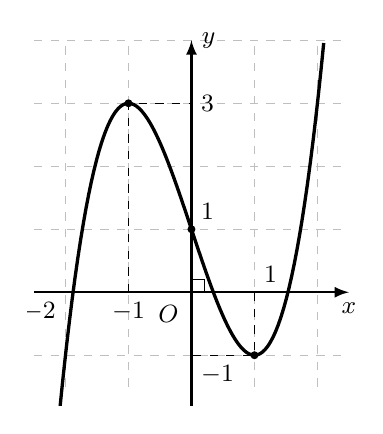
\begin{tikzpicture}[scale=0.8, >=latex]
    % 1. Giới hạn vùng hiển thị
    \clip (-2.6, -1.8) rectangle (2.6, 4.2);

    % 2. Lưới ô vuông (Grid) màu xám nét đứt
    \draw[gray!50, dashed, step=1] (-2.5, -1.5) grid (2.5, 4);

    % 3. Trục tọa độ Oxy màu đen
    \draw[->, thick, black] (-2.5, 0) -- (2.5, 0) node[below] {\small $x$};
    \draw[->, thick, black] (0, -1.8) -- (0, 4.0) node[right] {\small $y$};
    \node[below left] at (-0.05, -0.05) {\small $O$};

    % Ký hiệu góc vuông tại gốc tọa độ O
    \draw[black] (0.2, 0) -- (0.2, 0.2) -- (0, 0.2);

    % 4. Các đường dóng nét đứt tại cực trị (-1; 3) và (1; -1)
    \draw[dashed, black] (-1, 0) -- (-1, 3) -- (0, 3);
    \draw[dashed, black] (1, 0) -- (1, -1) -- (0, -1);

    % 5. Đồ thị hàm số bậc ba y = x^3 - 3x + 1
    \draw[very thick, black, domain=-2.1:2.1, samples=100] 
        plot (\x, {\x*\x*\x - 3*\x + 1});

    % 6. Đánh dấu các điểm nút đặc biệt (màu đen)
    \fill[black] (-1, 3) circle (1.8pt);
    \fill[black] (1, -1) circle (1.8pt);
    \fill[black] (0, 1) circle (1.8pt);

    % 7. Nhãn số và tọa độ trên các trục
    % Trên trục Ox
    \node[below left] at (-2, 0) {\small $-2$};
    \node[below] at (-1, 0) {\small $-1$};
    \node[above right] at (1, 0) {\small $1$};

    % Trên trục Oy
    \node[right] at (0, 3) {\small $3$};
    \node[above right] at (0, 1) {\small $1$};
    \node[below right] at (0, -1) {\small $-1$};
\end{tikzpicture}
\end{center}
}{
    \textbf{a)} & Trong các số \( a, b, c, d \) có ba giá trị dương.
    & \textcolor{amberorange}{$\bigcirc$} & \textcolor{amberorange}{$\bigcirc$} \\ \hline
    
    \textbf{b)} & Hàm số đạt giá trị lớn nhất trên \((-2;1)\) bằng 3.
    & \textcolor{amberorange}{$\bigcirc$} & \textcolor{amberorange}{$\bigcirc$} \\ \hline
    
    \textbf{c)} & Tâm đối xứng của đồ thị hàm số có hoành độ bằng 1.
    & \textcolor{amberorange}{$\bigcirc$} & \textcolor{amberorange}{$\bigcirc$} \\ \hline
    
    \textbf{d)} & Phương trình \( f(f(x)) = \dfrac{5}{2} \) có sáu nghiệm phân biệt.
    & \textcolor{amberorange}{$\bigcirc$} & \textcolor{amberorange}{$\bigcirc$} \\
}

\questionTrueFalse{0}{34}{Cho hàm số \( y = f(x) = \dfrac{x^2 + bx + c}{x - 2} \) có đạo hàm \( f'(x) \). Đồ thị của hàm số \( f'(x) \) như hình vẽ sau:

\begin{center}
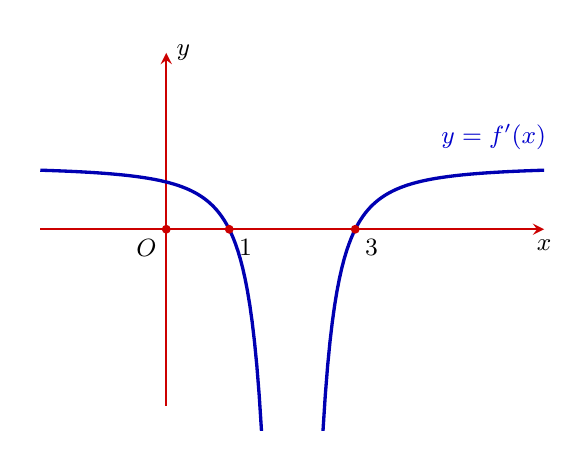
\begin{tikzpicture}[scale=0.8, >=latex]
    % 1. Giới hạn vùng hiển thị
    \clip (-2.2, -3.2) rectangle (6.2, 3.2);

    % 2. Trục tọa độ Oxy màu đỏ
    \draw[->, >=stealth, thick, red!80!black] (-2.0, 0) -- (6.0, 0) node[below, black] {\small $x$};
    \draw[->, >=stealth, thick, red!80!black] (0, -2.8) -- (0, 2.8) node[right, black] {\small $y$};

    % 3. Đồ thị đạo hàm y = 1 - 1/(x-2)^2 (màu xanh lam)
    % Nhánh trái (x < 2)
    \draw[very thick, blue!70!black, domain=-2.0:1.7, samples=100] 
        plot (\x, {1 - 1/((\x - 2)*(\x - 2))});
    % Nhánh phải (x > 2)
    \draw[very thick, blue!70!black, domain=2.3:6.0, samples=100] 
        plot (\x, {1 - 1/((\x - 2)*(\x - 2))});

    % 4. Các điểm nút màu đỏ và nhãn giao điểm
    % Gốc tọa độ O
    \fill[red!80!black] (0, 0) circle (2pt);
    \node[below left, black] at (0, 0) {\small $O$};

    % Giao điểm x = 1
    \fill[red!80!black] (1, 0) circle (2pt);
    \node[below right, black] at (1, 0) {\small $1$};

    % Giao điểm x = 3
    \fill[red!80!black] (3, 0) circle (2pt);
    \node[below right, black] at (3, 0) {\small $3$};

    % 5. Nhãn y = f'(x) màu xanh dương
    \node[blue!80!black, above] at (5.2, 1.1) {\small $y = f'(x)$};
\end{tikzpicture}
\end{center}
}{
    \textbf{a)} & Phương trình \( f'(x) = 0 \) có hai nghiệm \( x = 1 \) và \( x = 3 \).
    & \textcolor{amberorange}{$\bigcirc$} & \textcolor{amberorange}{$\bigcirc$} \\ \hline
    
    \textbf{b)} & Hàm số \( y = f(x) \) nghịch biến trên khoảng \((1; 3)\).
    & \textcolor{amberorange}{$\bigcirc$} & \textcolor{amberorange}{$\bigcirc$} \\ \hline
    
    \textbf{c)} & Hàm số \( y = f(x) \) đạt cực đại tại \( x = 1 \) và đạt cực tiểu tại \( x = 3 \).
    & \textcolor{amberorange}{$\bigcirc$} & \textcolor{amberorange}{$\bigcirc$} \\ \hline
    
    \textbf{d)} & Nếu \( f(0) = 1 \) thì \( \max_{[3;4]} f(x) = 6 \).
    & \textcolor{amberorange}{$\bigcirc$} & \textcolor{amberorange}{$\bigcirc$} \\
}

\questionTrueFalse{0}{35}{Cho hàm số bậc bốn \( y = f(x) \). Hàm số \( y = f'(x) \) có đồ thị như hình vẽ

\begin{center}
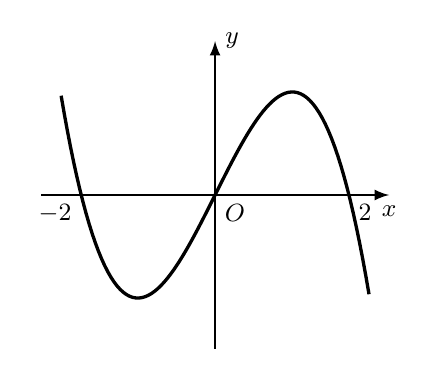
\begin{tikzpicture}[scale=0.85, >=latex]
    % 1. Giới hạn vùng hiển thị
    \clip (-2.8, -2.5) rectangle (2.8, 2.5);

    % 2. Trục tọa độ Oxy màu đen
    \draw[->, thick, black] (-2.6, 0) -- (2.6, 0) node[below] {\small $x$};
    \draw[->, thick, black] (0, -2.3) -- (0, 2.3) node[right] {\small $y$};
    \node[below right] at (0,0) {\small $O$};

    % 3. Đồ thị hàm số y = f'(x) = -x^3/2 + 2x (hoặc dạng tương đương)
    \draw[very thick, black, domain=-2.3:2.3, samples=100] 
        plot (\x, {-0.5*\x*\x*\x + 2*\x});

    % 4. Đánh dấu các nghiệm trên trục Ox
    \node[below left] at (-2, 0) {\small $-2$};
    \node[below right] at (2, 0) {\small $2$};
\end{tikzpicture}
\end{center}
}{
    \textbf{a)} & Hàm số \( y = f(x) \) nghịch biến trên khoảng \((-\infty; -2)\).
    & \textcolor{amberorange}{$\bigcirc$} & \textcolor{amberorange}{$\bigcirc$} \\ \hline
    
    \textbf{b)} & Hàm số \( y = f(x) \) có ba điểm cực trị.
    & \textcolor{amberorange}{$\bigcirc$} & \textcolor{amberorange}{$\bigcirc$} \\ \hline
    
    \textbf{c)} & Giá trị nhỏ nhất của hàm số \( y = f(x) \) trên đoạn \([-2; 2]\) là \( f(0) \).
    & \textcolor{amberorange}{$\bigcirc$} & \textcolor{amberorange}{$\bigcirc$} \\ \hline
    
    \textbf{d)} & Biết \( f(0) > 0 \) khi đó phương trình \( f(x) = 0 \) có tối đa ba nghiệm.
    & \textcolor{amberorange}{$\bigcirc$} & \textcolor{amberorange}{$\bigcirc$} \\
}


\questionTrueFalse{0}{36}{Cho hàm số \( y = \dfrac{x^2 + x + 1}{x + 1} \)}{
    \textbf{a)} & Hàm số có tập xác định là \( D = \mathbb{R} \).
    & \textcolor{amberorange}{$\bigcirc$} & \textcolor{amberorange}{$\bigcirc$} \\ \hline
    
    \textbf{b)} & \( y' = \dfrac{x^2 - 2x}{(x + 1)^2}, \, \forall x \neq -1 \).
    & \textcolor{amberorange}{$\bigcirc$} & \textcolor{amberorange}{$\bigcirc$} \\ \hline
    
    \textbf{c)} & Hàm số có bảng biến thiên như sau:
    \begin{center}
    
\begin{tikzpicture}
        \tkzTabInit[lgt=0.8, espcl=1.6]
        {$x$ /0.5, $y'$ /0.5, $y$ /1.5}
        {$-\infty$, $-2$, $-1$, $0$, $+\infty$}
        \tkzTabLine{, +, 0, -, d, -, 0, +, }
        \tkzTabVar{-/ $-\infty$ / ,+/$-3$, -D+/ $-\infty$ / $+\infty$ / , -/ $1$ / , +/ $+\infty$ /}
    \end{tikzpicture}
    \end{center}
    & \textcolor{amberorange}{$\bigcirc$} & \textcolor{amberorange}{$\bigcirc$} \\ \hline
    
    \textbf{d)} & Khoảng cách giữa 2 điểm cực trị của đồ thị hàm số là \( 2\sqrt{5} \).
    & \textcolor{amberorange}{$\bigcirc$} & \textcolor{amberorange}{$\bigcirc$} \\
}

\questionTrueFalse{0}{37}{Cho hàm số \( y = f(x) = x^3 - 3x \). Khi đó:}{
    \textbf{a)} & Hàm số đồng biến trên khoảng \((-1; 1)\).
    & \textcolor{amberorange}{$\bigcirc$} & \textcolor{amberorange}{$\bigcirc$} \\ \hline
    
    \textbf{b)} & Hàm số có 2 điểm cực trị.
    & \textcolor{amberorange}{$\bigcirc$} & \textcolor{amberorange}{$\bigcirc$} \\ \hline
    
    \textbf{c)} & Giá trị lớn nhất của hàm số \( y = f(x) + 2 \) trên đoạn \([0; 2]\) bằng 4.
    & \textcolor{amberorange}{$\bigcirc$} & \textcolor{amberorange}{$\bigcirc$} \\ \hline
    
    \textbf{d)} & Có duy nhất một giá trị của tham số thực \( m \) sao cho giá trị lớn nhất của hàm số \( y = |f(x) + m| \) trên đoạn \([0; 2]\) bằng 3.
    & \textcolor{amberorange}{$\bigcirc$} & \textcolor{amberorange}{$\bigcirc$} \\
}

\questionTrueFalse{0}{38}{Cho hàm số \( y = f(x) = \dfrac{x^2 - x + 2}{x - 2} \) có đồ thị \( (C) \).}{
    \textbf{a)} & Tiệm cận đứng của đồ thị \( (C) \) là \( x = 2 \).
    & \textcolor{amberorange}{$\bigcirc$} & \textcolor{amberorange}{$\bigcirc$} \\ \hline
    
    \textbf{b)} & Hàm số đồng biến trên \( (0; 2) \).
    & \textcolor{amberorange}{$\bigcirc$} & \textcolor{amberorange}{$\bigcirc$} \\ \hline
    
    \textbf{c)} & Đường thẳng \( y = x + 1 \) là tiệm cận xiên của đồ thị \( (C) \).
    & \textcolor{amberorange}{$\bigcirc$} & \textcolor{amberorange}{$\bigcirc$} \\ \hline
    
    \textbf{d)} & Có 2024 giá trị nguyên của \( m \in [0; 2025] \) để đường thẳng \( y = m \) cắt đồ thị \( (C) \) tại hai điểm phân biệt.
    & \textcolor{amberorange}{$\bigcirc$} & \textcolor{amberorange}{$\bigcirc$} \\
}

\questionTrueFalse{0}{39}{Số dân của một thị trấn sau \( t \) năm kể từ năm 1970 được ước tính bởi công thức  
\(f(t) = \dfrac{26t + 10}{t + 5}\) 
(\( f(t) \) được tính bằng nghìn người).}{
    \textbf{a)} & Số dân của thị trấn vào đầu năm 1980 là 18 nghìn người.
    & \textcolor{amberorange}{$\bigcirc$} & \textcolor{amberorange}{$\bigcirc$} \\ \hline
    
    \textbf{b)} & Số dân của thị trấn vào đầu năm 1995 là 23 nghìn người.
    & \textcolor{amberorange}{$\bigcirc$} & \textcolor{amberorange}{$\bigcirc$} \\ \hline
    
    \textbf{c)} & Xem \( f \) là một hàm số xác định trên nửa khoảng \([0; +\infty)\). Vậy hàm số đồng biến trên \([0; +\infty)\).
    & \textcolor{amberorange}{$\bigcirc$} & \textcolor{amberorange}{$\bigcirc$} \\ \hline
    
    \textbf{d)} & Đạo hàm của hàm số \( f \) biểu thị tốc độ tăng dân số của thị trấn (tính bằng nghìn người/năm).  
    Vào năm 1998 thì tốc độ tăng dân số là 0,125 nghìn người/năm.
    & \textcolor{amberorange}{$\bigcirc$} & \textcolor{amberorange}{$\bigcirc$} \\
}

\questionTrueFalse{0}{40}{Cho hàm số  
\(f(x) = e^x - 2x + e.\)
Xét tính đúng sai các mệnh đề sau:}{
    \textbf{a)} & Tập xác định của hàm số \( f(x) \) là \( D = \mathbb{R} \).
    & \textcolor{amberorange}{$\bigcirc$} & \textcolor{amberorange}{$\bigcirc$} \\ \hline
    
    \textbf{b)} & Đạo hàm của hàm số \( f(x) \) là  
    \(f'(x) = e^x - 2\).
    & \textcolor{amberorange}{$\bigcirc$} & \textcolor{amberorange}{$\bigcirc$} \\ \hline
    
    \textbf{c)} & Giá trị lớn nhất của hàm số \( f(x) \) trên đoạn \([0; 2]\) bằng \( e^2 + e \).
    & \textcolor{amberorange}{$\bigcirc$} & \textcolor{amberorange}{$\bigcirc$} \\ \hline
    
    \textbf{d)} & Đường cong \( y = f(x) \) cắt đường thẳng \( y = -2x \) tại hai điểm phân biệt.
    & \textcolor{amberorange}{$\bigcirc$} & \textcolor{amberorange}{$\bigcirc$} \\
}


\questionTrueFalse{0}{41}{Cho hàm số \( y = \dfrac{x-1}{x+2} \) có đồ thị \((C)\). Gọi \( I \) là giao điểm của hai tiệm cận của \((C)\).}{
    \textbf{a)} & Hàm số đồng biến trên \(\mathbb{R} \setminus \{-2\}\).
    & \textcolor{amberorange}{$\bigcirc$} & \textcolor{amberorange}{$\bigcirc$} \\ \hline
    
    \textbf{b)} & Hàm số có tâm đối xứng \( I(-2;1) \).
    & \textcolor{amberorange}{$\bigcirc$} & \textcolor{amberorange}{$\bigcirc$} \\ \hline
    
    \textbf{c)} & Phương trình tiếp tuyến của đồ thị \((C)\) tại điểm \( x = 1 \) là \( y = \dfrac{1}{3}x - \dfrac{1}{3} \).
    & \textcolor{amberorange}{$\bigcirc$} & \textcolor{amberorange}{$\bigcirc$} \\ \hline
    
    \textbf{d)} & Xét tam giác đều \( ABI \) có hai đỉnh \( A, B \) thuộc \((C)\), \( AB = 2\sqrt{3} \).
    & \textcolor{amberorange}{$\bigcirc$} & \textcolor{amberorange}{$\bigcirc$} \\
}

\questionTrueFalse{0}{42}{Cho hàm số \( y = f(x) = ax^3 + bx^2 + cx + d \) có bảng biến thiên như sau:

\begin{center}

\begin{tikzpicture}
    \tkzTabInit[lgt=1.5, espcl=2.5]
    {$x$ /1, $f'(x)$ /1, $f(x)$ /2.5}
    {$-\infty$, $1$, $3$, $+\infty$}
    \tkzTabLine{, -, 0, +, 0, -, }
    \tkzTabVar{+/ $+\infty$ / , -/ $2$ / , +/ $4$ / , -/ $-\infty$ /}
\end{tikzpicture}
\end{center}
}{
    \textbf{a)} & Hàm số có hệ số \( a < 0 \).
    & \textcolor{amberorange}{$\bigcirc$} & \textcolor{amberorange}{$\bigcirc$} \\ \hline
    
    \textbf{b)} & Đồ thị hàm số đi qua hai điểm \( (1; 2) \), \( (3; 4) \).
    & \textcolor{amberorange}{$\bigcirc$} & \textcolor{amberorange}{$\bigcirc$} \\ \hline
    
    \textbf{c)} & \( f'(x) = 0 \) tại các giá trị \( x = 2 \), \( x = 4 \).
    & \textcolor{amberorange}{$\bigcirc$} & \textcolor{amberorange}{$\bigcirc$} \\ \hline
    
    \textbf{d)} & Giá trị nhỏ nhất của hàm số trên \([2; 4]\) bằng \( \dfrac{7}{2} \).
    & \textcolor{amberorange}{$\bigcirc$} & \textcolor{amberorange}{$\bigcirc$} \\
}

\questionTrueFalse{0}{43}{Nhà máy \( A \) chuyên sản xuất một loại sản phẩm cho nhà máy \( B \). Hai nhà máy thỏa thuận rằng, hàng tháng nhà máy \( A \) cung cấp cho nhà máy \( B \) số lượng sản phẩm theo đơn đặt hàng của nhà máy \( B \) (tối đa 100 tấn sản phẩm). Biết rằng, nếu số lượng đặt hàng là \( x \) (tấn) sản phẩm thì giá bán cho mỗi tấn sản phẩm là \( P(x) = 45 - 0,001x^2 \) (triệu đồng) và chi phí để nhà máy \( A \) sản xuất được \( x \) (tấn) sản phẩm trong một tháng là \( C(x) = 100 + 30x \) (triệu đồng, gồm 100 triệu đồng chi phí cố định và 30 triệu đồng cho mỗi tấn sản phẩm).}{
    \textbf{a)} & Số tiền nhà máy \( A \) thu được khi bán 10 tấn sản phẩm cho nhà máy \( B \) là 500 triệu đồng.
    & \textcolor{amberorange}{$\bigcirc$} & \textcolor{amberorange}{$\bigcirc$} \\ \hline
    
    \textbf{b)} & Nhà máy \( A \) bán cho nhà máy \( B \) là 70 tấn sản phẩm mỗi tháng thì thu được lợi nhuận lớn nhất.
    & \textcolor{amberorange}{$\bigcirc$} & \textcolor{amberorange}{$\bigcirc$} \\ \hline
    
    \textbf{c)} & Chi phí để nhà máy \( A \) sản xuất 10 tấn sản phẩm trong một tháng là 400 triệu đồng.
    & \textcolor{amberorange}{$\bigcirc$} & \textcolor{amberorange}{$\bigcirc$} \\ \hline
    
    \textbf{d)} & Lợi nhuận nhà máy \( A \) thu được khi bán \( x \) (tấn) sản phẩm \( (0 \leq x \leq 100) \) cho nhà máy \( B \) là  
    \(H(x) = -0,001x^3 + 15x - 100\) (triệu đồng).
    & \textcolor{amberorange}{$\bigcirc$} & \textcolor{amberorange}{$\bigcirc$} \\
}

\questionTrueFalse{0}{44}{Cho hàm số \( y = \dfrac{x^2 + bx + c}{x + n} \) có đồ thị và hai đường tiệm cận \( d_1, d_2 \) như hình vẽ dưới đây.

\begin{center}
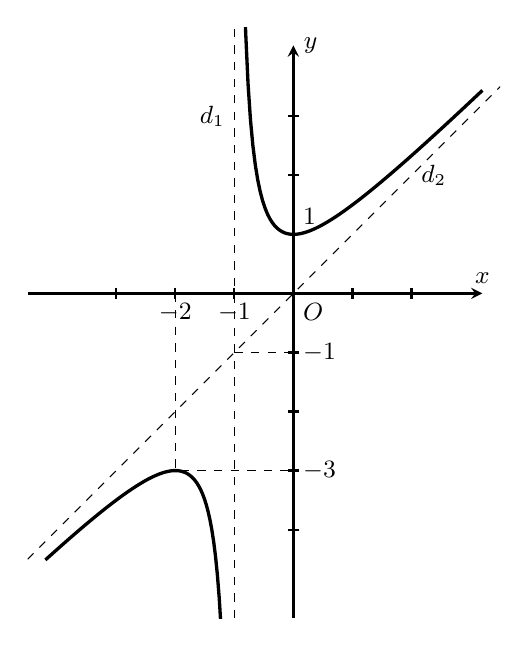
\begin{tikzpicture}[scale=0.75, >=latex]
    % 1. Giới hạn vùng hiển thị
    \clip (-4.5, -5.5) rectangle (3.5, 4.5);

    % 2. Các đường dóng nét đứt màu xanh lá cây tại điểm cực trị
    % Điểm cực tiểu (0; 1) và Cực đại (-2; -3)
    \draw[dashed ] (-2, 0) -- (-2, -3) -- (0, -3);
    \draw[dashed] (-1, -1) -- (0, -1);

    % 3. Đường tiệm cận d1 và d2 (nét đứt màu xanh lam)
    % Tiệm cận đứng d1: x = -1
    \draw[dashed] (-1, -5.5) -- (-1, 4.5);
    \node[ left] at (-1, 3.0) {\small $d_1$};

    % Tiệm cận xiên d2: y = x
    \draw[dashed, domain=-4.5:4.5] plot (\x, {\x});
    \node[,right] at (2.0, 2.0) {\small $d_2$};

    % 4. Đồ thị hàm số y = (x^2 + x + 1)/(x + 1) = x + 1/(x + 1) (màu xanh lá cây)
    % Nhánh trên (x > -1)
    \draw[very thick, domain=-0.85:3.2, samples=100] 
        plot (\x, {\x + 1/(\x + 1)});
    % Nhánh dưới (x < -1)
    \draw[very thick, domain=-4.2:-1.1, samples=100] 
        plot (\x, {\x + 1/(\x + 1)});

    % 5. Trục tọa độ Oxy màu đỏ (vẽ đè lên để hiển thị rõ)
    \draw[->, >=stealth, thick] (-4.5, 0) -- (3.2, 0) node[above] {\small $x$};
    \draw[->, >=stealth, thick] (0, -5.5) -- (0, 4.2) node[right] {\small $y$};

    % Các vạch chia trên trục Ox và Oy (màu đen)
    \foreach \x in {-3,-2,-1,1,2}
        \draw[thick, black] (\x, 0.1) -- (\x, -0.1);
    \foreach \y in {-4,-3,-2,-1,1,2,3}
        \draw[thick, black] (0.1, \y) -- (-0.1, \y);

    % 6. Các điểm đặc biệt và nhãn giá trị
    % Gốc tọa độ O
    \node[below right] at (0, 0) {\small $O$};

    % Nhãn hoành độ
    \node[below] at (-2, 0) {\small $-2$};
    \node[below] at (-1, 0) {\small $-1$};

    % Nhãn tung độ
    \node[above right] at (0, 1) {\small $1$};
    \node[right] at (0, -1) {\small $-1$};
    \node[right] at (0, -3) {\small $-3$};

\end{tikzpicture}
\end{center}
}{
    \textbf{a)} & Đồ thị hàm số có tiệm cận đứng là đường thẳng \( x = -1 \).
    & \textcolor{amberorange}{$\bigcirc$} & \textcolor{amberorange}{$\bigcirc$} \\ \hline
    
    \textbf{b)} & Hàm số đồng biến trên khoảng \( (0; +\infty) \).
    & \textcolor{amberorange}{$\bigcirc$} & \textcolor{amberorange}{$\bigcirc$} \\ \hline
    
    \textbf{c)} & Đồ thị hàm số có 2 trục đối xứng, trong đó có một trục đối xứng là đường thẳng \( y = (p + \sqrt{q})(x + 1) - r \) (\( p, q, r \) là các số nguyên). Khi đó \( p + q + r = 4 \).
    & \textcolor{amberorange}{$\bigcirc$} & \textcolor{amberorange}{$\bigcirc$} \\ \hline
    
    \textbf{d)} & Điểm \( M(1212; 2025) \) và hai điểm cực trị của đồ thị hàm số thẳng hàng.
    & \textcolor{amberorange}{$\bigcirc$} & \textcolor{amberorange}{$\bigcirc$} \\
}

\questionTrueFalse{0}{45}{Chi phí nhiên liệu của một chiếc tàu chạy trên sông được chia làm hai phần. Phần thứ nhất chi phí hết 1250 nghìn đồng trên 1 giờ. Phần thứ hai chi phí hết \(0,04x^3\) nghìn đồng trên 1 giờ nếu tàu chạy với vận tốc \( x \) km/giờ.}{
    \textbf{a)} & Khi tàu chạy với vận tốc 10 km/giờ thì chi phí nguyên liệu cho phần thứ nhất trên 1 km đường sông là 125 nghìn đồng.
    & \textcolor{amberorange}{$\bigcirc$} & \textcolor{amberorange}{$\bigcirc$} \\ \hline
    
    \textbf{b)} & Hàm số xác định tổng chi phí nguyên liệu trên 1 km đường sông khi tàu chạy với vận tốc \( x \) km/giờ là  
    \(f(x) = \dfrac{1250}{x} + 0,04x^2\) (nghìn đồng).
    & \textcolor{amberorange}{$\bigcirc$} & \textcolor{amberorange}{$\bigcirc$} \\ \hline
    
    \textbf{c)} & Khi tàu chạy với tốc độ 20 km/giờ thì tổng chi phí nguyên liệu trên 2 km đường sông là 78500 đồng.
    & \textcolor{amberorange}{$\bigcirc$} & \textcolor{amberorange}{$\bigcirc$} \\ \hline
    
    \textbf{d)} & Khi tàu chạy với vận tốc 25 km/giờ thì tổng chi phí nguyên liệu trên 1 km đường sông là nhỏ nhất.
    & \textcolor{amberorange}{$\bigcirc$} & \textcolor{amberorange}{$\bigcirc$} \\
}

\questionTrueFalse{0}{46}{Cho hàm số \( y = -x^3 + 3x^2 + 4 \) có đồ thị \((C)\).}{
    \textbf{a)} & Hàm số có đạo hàm là \( y' = -3x^2 + 6x \).
    & \textcolor{amberorange}{$\bigcirc$} & \textcolor{amberorange}{$\bigcirc$} \\ \hline
    
    \textbf{b)} & Hàm số đồng biến trên khoảng \((0; 2)\).
    & \textcolor{amberorange}{$\bigcirc$} & \textcolor{amberorange}{$\bigcirc$} \\ \hline
    
    \textbf{c)} & Đồ thị \((C)\) có hai điểm cực trị và đường thẳng qua hai điểm cực trị là \( 2x + y - 4 = 0 \).
    & \textcolor{amberorange}{$\bigcirc$} & \textcolor{amberorange}{$\bigcirc$} \\ \hline
    
    \textbf{d)} & Diện tích tam giác \( AOB \) bằng 4 trong đó \(A\) và \(B\) là hai điểm cực trị của \((C)\).
    & \textcolor{amberorange}{$\bigcirc$} & \textcolor{amberorange}{$\bigcirc$} \\
}


\questionTrueFalse{0}{47}{Từ một tấm bìa mỏng hình lục giác đều \( ABCDEF \) cạnh 4 cm, bên trong có một lục giác đều nhỏ hơn. Các đường chéo \( AD, BE, CF \) cắt nhau tại \( O \), cắt cạnh lục giác đều nhỏ tại \( M \) (như hình vẽ). Đặt \( OM = x \) (cm). Bạn Khôi cắt bỏ 6 tam giác cân bằng nhau có cạnh đáy là cạnh của lục giác đều ban đầu và đỉnh là đỉnh của lục giác đều nhỏ phía trong rồi gấp lên sao cho các đỉnh \( A, B, C, D, E, F \) trùng nhau tạo thành một khối chóp lục giác đều.

\begin{center}
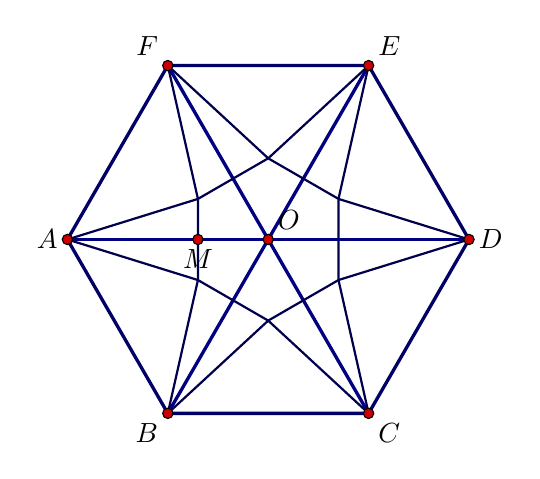
\begin{tikzpicture}[scale=0.85, >=latex]
    % 1. Định nghĩa các đỉnh của lục giác đều lớn ABCDEF (Bán kính R = 3)
    \path (180:3) coordinate (A)
          (240:3) coordinate (B)
          (300:3) coordinate (C)
          (0:3)   coordinate (D)
          (60:3)  coordinate (E)
          (120:3) coordinate (F);

    % Tâm O
    \coordinate (O) at (0,0);

    % Điểm M nằm trên đường chéo AD (đoạn AO)
    % Tỷ lệ x = OM/OA (ở đây chọn 0.35)
    \coordinate (M) at (-1.05, 0);

    % các đỉnh của lục giác nhỏ phía trong (xoay 30 độ để các cạnh vuông góc với đường chéo)
    \pgfmathsetmacro{\rsmall}{1.05 / cos(30)}
    \path (150:\rsmall) coordinate (P1)
          (210:\rsmall) coordinate (P2)
          (270:\rsmall) coordinate (P3)
          (330:\rsmall) coordinate (P4)
          (30:\rsmall)  coordinate (P5)
          (90:\rsmall)  coordinate (P6);

    % 2. Vẽ cạnh lục giác đều lớn ngoài cùng ABCDEF (màu tím đậm)
    \draw[very thick, blue!40!black] (A) -- (B) -- (C) -- (D) -- (E) -- (F) -- cycle;

    % 3. Vẽ 3 đường chéo chính AD, BE, CF (màu xanh tím)
    \draw[very thick, blue!50!black] (A) -- (D);
    \draw[very thick, blue!50!black] (B) -- (E);
    \draw[very thick, blue!50!black] (C) -- (F);

    % 4. Vẽ các nếp gấp từ đỉnh lục giác nhỏ đến các đỉnh A, B, C, D, E, F
    \draw[thick, blue!30!black] (P1) -- (A);
    \draw[thick, blue!30!black] (P1) -- (F);
    
    \draw[thick, blue!30!black] (P2) -- (A);
    \draw[thick, blue!30!black] (P2) -- (B);

    \draw[thick, blue!30!black] (P3) -- (B);
    \draw[thick, blue!30!black] (P3) -- (C);

    \draw[thick, blue!30!black] (P4) -- (C);
    \draw[thick, blue!30!black] (P4) -- (D);

    \draw[thick, blue!30!black] (P5) -- (D);
    \draw[thick, blue!30!black] (P5) -- (E);

    \draw[thick, blue!30!black] (P6) -- (E);
    \draw[thick, blue!30!black] (P6) -- (F);

    % 5. Vẽ cạnh của lục giác nhỏ phía trong
    \draw[thick, blue!30!black] (P1) -- (P2) -- (P3) -- (P4) -- (P5) -- (P6) -- cycle;

    % 6. Đánh dấu các điểm nút màu đỏ với viền đen
    \foreach \pt in {A,B,C,D,E,F,O,M} {
        \fill[red!80!black] (\pt) circle (2.2pt);
        \draw[black, thin] (\pt) circle (2.2pt);
    }

    % 7. Nhãn các điểm
    \node[left, font=\bfseries\itshape] at (A) {$A$};
    \node[below left, font=\bfseries\itshape] at (B) {$B$};
    \node[below right, font=\bfseries\itshape] at (C) {$C$};
    \node[right, font=\bfseries\itshape] at (D) {$D$};
    \node[above right, font=\bfseries\itshape] at (E) {$E$};
    \node[above left, font=\bfseries\itshape] at (F) {$F$};
    \node[above right, font=\bfseries\itshape] at (O) {$O$};
    \node[below, font=\bfseries\itshape] at (M) {$M$};
\end{tikzpicture}
\end{center}
}{
    \textbf{a)} & Tam giác \( OAB \) đều có cạnh bằng 4 cm.
    & \textcolor{amberorange}{$\bigcirc$} & \textcolor{amberorange}{$\bigcirc$} \\ \hline
    
    \textbf{b)} & Cạnh đáy của khối chóp lục giác đều bằng  
    \(\dfrac{x\sqrt{3}}{6}\) (cm).
    & \textcolor{amberorange}{$\bigcirc$} & \textcolor{amberorange}{$\bigcirc$} \\ \hline
    
    \textbf{c)} & Đường cao của khối chóp lục giác đều bằng  
    \(\sqrt{16 - 8x}\) (cm).
    & \textcolor{amberorange}{$\bigcirc$} & \textcolor{amberorange}{$\bigcirc$} \\ \hline
    
    \textbf{d)} & Thể tích lớn nhất của khối chóp lục giác đều có thể đạt được là  
    \(\dfrac{256\sqrt{10}}{375} \ (cm^3)\).
    & \textcolor{amberorange}{$\bigcirc$} & \textcolor{amberorange}{$\bigcirc$} \\
}


\questionTrueFalse{0}{48}{Cho hàm số \( y = f(x) = \dfrac{x^2 - 2x + 5}{x - 1} \) có đồ thị là \((C)\).}{
    \textbf{a)} & Hàm số đồng biến trên khoảng \((2; +\infty)\).
    & \textcolor{amberorange}{$\bigcirc$} & \textcolor{amberorange}{$\bigcirc$} \\ \hline
    
    \textbf{b)} & Gọi \(x_1, x_2\) là hai nghiệm của phương trình \(f'(x) = 0\). Khi đó \(x_1^2 + x_2^2 = 10\).
    & \textcolor{amberorange}{$\bigcirc$} & \textcolor{amberorange}{$\bigcirc$} \\ \hline
    
    \textbf{c)} & Hàm số có tập xác định là \(D = \mathbb{R} \setminus \{1\}\).
    & \textcolor{amberorange}{$\bigcirc$} & \textcolor{amberorange}{$\bigcirc$} \\ \hline
    
    \textbf{d)} & Gọi \((d)\) là tiếp tuyến với đồ thị hàm số \((C)\) tại điểm \(M(2; 5)\). Biết \((d)\) cắt hai đường tiệm cận của \((C)\) tại hai điểm \(A, B\). Gọi \(I\) là tâm đối xứng của \((C)\). Diện tích tam giác \(IAB\) bằng 8 (đvdt).
    & \textcolor{amberorange}{$\bigcirc$} & \textcolor{amberorange}{$\bigcirc$} \\
}

\questionTrueFalse{0}{49}{Cho hàm số \( f(x) = \dfrac{ax^2 + bx + c}{x + d} \) có bảng biến thiên như hình vẽ dưới đây

\begin{center}

\begin{tikzpicture}
    \tkzTabInit[lgt=1.5, espcl=2.5]
    {$x$ /1, $f'(x)$ /1, $f(x)$ /2.5}
    {$-\infty$, $0$, $2$, $4$, $+\infty$}
    \tkzTabLine{, -, 0, +, d, +, 0, -, }
    \tkzTabVar{+/ $+\infty$ / , -/ $2$ / , +D-/ $+\infty$ / $-\infty$, +/ $-6$ / , -/ $-\infty$ /}
\end{tikzpicture}
\end{center}
}{
    \textbf{a)} & Phương trình đường thẳng qua hai điểm cực trị là \(\Delta : 2x + y - 2 = 0\).
    & \textcolor{amberorange}{$\bigcirc$} & \textcolor{amberorange}{$\bigcirc$} \\ \hline
    
    \textbf{b)} & Hàm số \( f(x) \) có ba điểm cực trị.
    & \textcolor{amberorange}{$\bigcirc$} & \textcolor{amberorange}{$\bigcirc$} \\ \hline
    
    \textbf{c)} & \( a + b + c + d = -5 \).
    & \textcolor{amberorange}{$\bigcirc$} & \textcolor{amberorange}{$\bigcirc$} \\ \hline
    
    \textbf{d)} & Hàm số \( f(x) \) đồng biến trên khoảng \((1;3)\).
    & \textcolor{amberorange}{$\bigcirc$} & \textcolor{amberorange}{$\bigcirc$} \\
}


\questionTrueFalse{0}{50}{Cho hàm số \( y = -x^3 + 3x^2 + 4 \) có đồ thị \( (C) \). Xét tính đúng sai của các mệnh đề sau:}{
    \textbf{a)} & Đồ thị \( (C) \) có hai điểm cực trị và phương trình đường thẳng đi qua hai điểm cực trị là  
    \( 2x + y - 4 = 0 \).
    & \textcolor{amberorange}{$\bigcirc$} & \textcolor{amberorange}{$\bigcirc$} \\ \hline
    
    \textbf{b)} & Tập xác định của hàm số là \( D = \mathbb{R} \) và \( y' = -3x^3 + 6x \).
    & \textcolor{amberorange}{$\bigcirc$} & \textcolor{amberorange}{$\bigcirc$} \\ \hline
    
    \textbf{c)} & Hàm số đồng biến trên khoảng \( (0; 2) \).
    & \textcolor{amberorange}{$\bigcirc$} & \textcolor{amberorange}{$\bigcirc$} \\ \hline
    
    \textbf{d)} & Diện tích của tam giác \( OAB \) bằng 4, với \( O \) là gốc tọa độ và \( A, B \) là các điểm cực trị của \( (C) \).
    & \textcolor{amberorange}{$\bigcirc$} & \textcolor{amberorange}{$\bigcirc$} \\
}

\questionTrueFalse{0}{51}{Cho hàm số \( y = \dfrac{2x^2 - 5x + 7}{x - 5} \) có đồ thị \( (C) \).}{
    \textbf{a)} & Tiếp tuyến của đồ thị \( (C) \) tại điểm \( M(3; -5) \) cắt đường tiệm cận đứng và tiệm cận xiên lần lượt tại \( P, Q \). Diện tích tam giác \( OPQ \) là 52 với \( O \) là gốc tọa độ.
    & \textcolor{amberorange}{$\bigcirc$} & \textcolor{amberorange}{$\bigcirc$} \\ \hline
    
    \textbf{b)} & Tổng tất cả các giá trị cực trị của hàm số bằng 30.
    & \textcolor{amberorange}{$\bigcirc$} & \textcolor{amberorange}{$\bigcirc$} \\ \hline
    
    \textbf{c)} & Hàm số nghịch biến trên khoảng \((-1; 5)\).
    & \textcolor{amberorange}{$\bigcirc$} & \textcolor{amberorange}{$\bigcirc$} \\ \hline
    
    \textbf{d)} & Đường tiệm cận xiên của đồ thị \( (C) \) có phương trình \( y = 2x - 5 \).
    & \textcolor{amberorange}{$\bigcirc$} & \textcolor{amberorange}{$\bigcirc$} \\
}

\questionTrueFalse{0}{52}{Cho hàm số \( y = f(x) \) có đạo hàm trên \( \mathbb{R} \) và đồ thị như hình vẽ.

\begin{center}
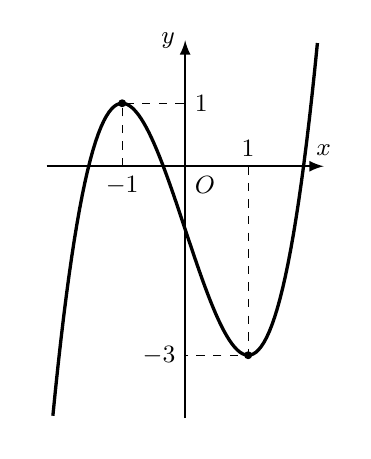
\begin{tikzpicture}[scale=0.8, >=latex]
    % 1. Giới hạn vùng hiển thị
    \clip (-2.5, -4.2) rectangle (2.5, 2.2);

    % 2. Trục tọa độ Oxy màu đen
    \draw[->, thick, black] (-2.2, 0) -- (2.2, 0) node[above] {\small $x$};
    \draw[->, thick, black] (0, -4.0) -- (0, 2.0) node[left] {\small $y$};
    \node[below right] at (0, 0) {\small $O$};

    % 3. Đường dóng nét đứt màu đen
    % Tại điểm cực đại (-1; 1)
    \draw[dashed, black] (-1, 0) -- (-1, 1) -- (0, 1);
    % Tại điểm cực tiểu (1; -3)
    \draw[dashed, black] (1, 0) -- (1, -3) -- (0, -3);

    % 4. Đồ thị hàm số y = x^3 - 3x - 1
    \draw[very thick, black, domain=-2.1:2.1, samples=100] 
        plot (\x, {\x*\x*\x - 3*\x - 1});

    % 5. Đánh dấu các điểm cực trị (màu đen)
    \fill[black] (-1, 1) circle (1.8pt);
    \fill[black] (1, -3) circle (1.8pt);

    % 6. Nhãn tọa độ trên các trục
    % Trên trục Ox
    \node[below] at (-1, 0) {\small $-1$};
    \node[above] at (1, 0) {\small $1$};

    % Trên trục Oy
    \node[right] at (0, 1) {\small $1$};
    \node[left] at (0, -3) {\small $-3$};
\end{tikzpicture}
\end{center}
}{
    \textbf{a)} & Hàm số nghịch biến trên khoảng \((-1; 1)\).
    & \textcolor{amberorange}{$\bigcirc$} & \textcolor{amberorange}{$\bigcirc$} \\ \hline
    
    \textbf{b)} & Hàm số đạt cực tiểu tại điểm \( x_0 = 1 \).
    & \textcolor{amberorange}{$\bigcirc$} & \textcolor{amberorange}{$\bigcirc$} \\ \hline
    
    \textbf{c)} & Đạo hàm của hàm số nhận giá trị dương trên khoảng \((-\infty; -1)\).
    & \textcolor{amberorange}{$\bigcirc$} & \textcolor{amberorange}{$\bigcirc$} \\ \hline
    
    \textbf{d)} & Giá trị nhỏ nhất của hàm số trên đoạn \([-1; 0]\) bằng \(-3\).
    & \textcolor{amberorange}{$\bigcirc$} & \textcolor{amberorange}{$\bigcirc$} \\
}

\questionTrueFalse{0}{53}{Cho hàm số \( y = \dfrac{x^2 - 3x + 5}{x + 1} \) có đồ thị \( (C) \).}{
    \textbf{a)} & Đường thẳng \( y = x + 1 \) là tiệm cận xiên của đồ thị \( (C) \).
    & \textcolor{amberorange}{$\bigcirc$} & \textcolor{amberorange}{$\bigcirc$} \\ \hline
    
    \textbf{b)} & Đồ thị \( (C) \) có tiệm cận đứng là đường thẳng \( x = -1 \).
    & \textcolor{amberorange}{$\bigcirc$} & \textcolor{amberorange}{$\bigcirc$} \\ \hline
    
    \textbf{c)} & Đường thẳng đi qua điểm cực đại và điểm cực tiểu của đồ thị hàm số là \( y = 2x + 3 \).
    & \textcolor{amberorange}{$\bigcirc$} & \textcolor{amberorange}{$\bigcirc$} \\ \hline
    
    \textbf{d)} & Hàm số nghịch biến trên khoảng \((-4; -1)\) và \((-1; 2)\).
    & \textcolor{amberorange}{$\bigcirc$} & \textcolor{amberorange}{$\bigcirc$} \\
}

\questionTrueFalse{0}{54}{Cho hàm số \( y = \dfrac{ax^2 + bx + c}{x + d} \) (\( a \neq 0 \)) có đồ thị là đường cong \( C \). Các đường thẳng \( d_1, d_2 \) lần lượt là tiệm cận đứng và tiệm cận xiên của đường cong \( C \) như hình vẽ.

\begin{center}
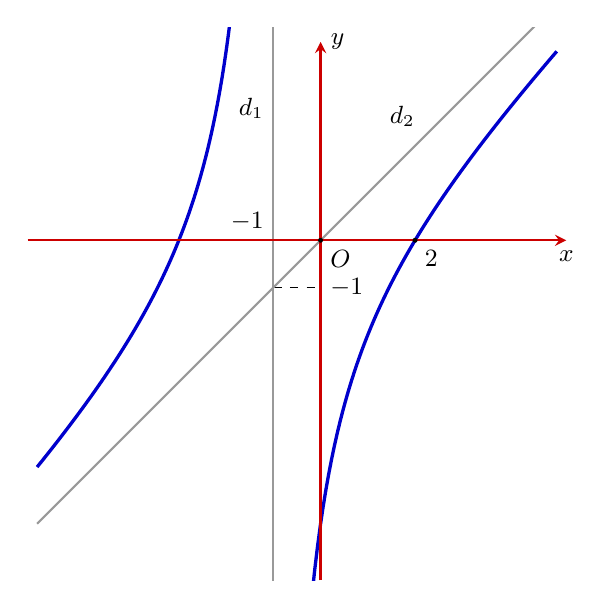
\begin{tikzpicture}[scale=0.6, >=latex]
    % 1. Giới hạn vùng hiển thị
    \clip (-6.2, -7.2) rectangle (5.5, 4.5);

    % 2. Các đường dóng nét đứt màu đen
    \draw[dashed, black] (-1, -1) -- (0, -1);

    % 3. Đường tiệm cận d1 và d2
    % Tiệm cận đứng d1: x = -1 (màu xám)
    \draw[thick, gray!80] (-1, -7.5) -- (-1, 6.5);
    \node[black, left] at (-1, 2.8) {\small $d_1$};

    % Tiệm cận xiên d2: y = x (màu xám)
    \draw[thick, gray!80, domain=-6:5.5] plot (\x, {\x});
    \node[black, above left] at (2.2, 2.2) {\small $d_2$};

    % 4. Đồ thị hàm số y = (x^2 - 2)/(x + 1) = x - 1 - 1/(x + 1) (màu xanh lam)
    % Nhánh trái (x < -1)
    \draw[very thick, blue!80!black, domain=-6:-1.1, samples=100] 
        plot (\x, {\x-6/(\x+1)});
    % Nhánh phải (x > -1)
    \draw[very thick, blue!80!black, domain=-0.9:5, samples=100] 
         plot (\x, {\x-6/(\x+1)});

    % 5. Trục tọa độ Oxy màu đỏ (vẽ đè lên trên đồ thị)
    \draw[->, >=stealth, thick, red!80!black] (-6.2, 0) -- (5.2, 0) node[below, black] {\small $x$};
    \draw[->, >=stealth, thick, red!80!black] (0, -7.2) -- (0, 4.2) node[right, black] {\small $y$};

    % 6. Các nhãn giá trị và tọa độ
    % Gốc tọa độ O
    \fill[black] (0, 0) circle (1.5pt);
    \node[below right, black] at (0, 0) {\small $O$};

    % Hoành độ x = -1
    \node[above left, black] at (-1, 0) {\small $-1$};

    % Tung độ y = -1
    \node[right, black] at (0, -1) {\small $-1$};

    % Giao điểm với trục Ox tại x = 2
    \fill[black] (2, 0) circle (1.5pt);
    \node[below right, black] at (2, 0) {\small $2$};
\end{tikzpicture}
\end{center}
}{
    \textbf{a)} & Đồ thị \( C \) đi qua điểm có tọa độ \( (0; 2) \).
    & \textcolor{amberorange}{$\bigcirc$} & \textcolor{amberorange}{$\bigcirc$} \\ \hline
    
    \textbf{b)} & Đồ thị \( C \) có tiệm cận đứng là đường thẳng \( x = -1 \).
    & \textcolor{amberorange}{$\bigcirc$} & \textcolor{amberorange}{$\bigcirc$} \\ \hline
    
    \textbf{c)} & Đồ thị \( C \) có tiệm cận xiên là đường thẳng \( y = x \).
    & \textcolor{amberorange}{$\bigcirc$} & \textcolor{amberorange}{$\bigcirc$} \\ \hline
    
    \textbf{d)} & Giá trị của tổng \( a + b + c + d \) là một số âm.
    & \textcolor{amberorange}{$\bigcirc$} & \textcolor{amberorange}{$\bigcirc$} \\
}


\questionTrueFalse{0}{55}{Cho hàm số \( y = f(x) = x^3 + bx^2 + cx + 2 \) đạt cực trị bằng 0 tại \( x = 1 \) (với \( b \) và \( c \) là hằng số).}{
    \textbf{a)} & Đồ thị hàm số đi qua điểm \( I(2;4) \).
    & \textcolor{amberorange}{$\bigcirc$} & \textcolor{amberorange}{$\bigcirc$} \\ \hline
    
    \textbf{b)} & Điểm \( M \) thay đổi trên đường thẳng nối 2 điểm cực trị của đồ thị hàm số. Với \( O \) là gốc toạ độ thì độ dài \( OM \) nhỏ nhất bằng \( \dfrac{4}{5} \).
    & \textcolor{amberorange}{$\bigcirc$} & \textcolor{amberorange}{$\bigcirc$} \\ \hline
    
    \textbf{c)} & \( f'(x) = 3x^2 + 2bx + c, \, \forall x \in \mathbb{R} \).
    & \textcolor{amberorange}{$\bigcirc$} & \textcolor{amberorange}{$\bigcirc$} \\ \hline
    
    \textbf{d)} & Đồ thị hàm số có hai điểm cực trị là \( A, B \). Độ dài \( AB = 5\sqrt{2} \).
    & \textcolor{amberorange}{$\bigcirc$} & \textcolor{amberorange}{$\bigcirc$} \\
}

\questionTrueFalse{0}{56}{Một hộ gia đình muốn xây dựng một bể chứa nước có dạng hình hộp chữ nhật không nắp, thể tích \( V = 12m^3 \). Đáy bể là hình chữ nhật có chiều dài gấp đôi chiều rộng. Giá thuê nhân công và vật liệu xây đáy là 500 nghìn đồng /\( m^2 \), xây thành bể là 300 nghìn đồng /\( m^2 \). Gọi \( x \) là chiều rộng của đáy bể, \( h \) là chiều cao của bể (\( x > 0, h > 0 \), đơn vị: \( m \)).}{
    \textbf{a)} & Tổng chi phí xây dựng bể nước là  
    \(T(x) = 500x^2 + \dfrac{10800}{x}\) (nghìn đồng).
    & \textcolor{amberorange}{$\bigcirc$} & \textcolor{amberorange}{$\bigcirc$} \\ \hline
    
    \textbf{b)} & Chiều cao của bể nước tính theo \( x \) là  
    \(h = \dfrac{6}{x^2} \, (m)\).
    & \textcolor{amberorange}{$\bigcirc$} & \textcolor{amberorange}{$\bigcirc$} \\ \hline
    
    \textbf{c)} & Thể tích của bể được tính bằng công thức  
    \(V = 2x^2h \, (m^3)\).
    & \textcolor{amberorange}{$\bigcirc$} & \textcolor{amberorange}{$\bigcirc$} \\ \hline
    
    \textbf{d)} & Tổng chi phí tối thiểu để xây dựng bể là 9234 (nghìn đồng) (không làm tròn kết quả các phép toán trung gian, chỉ làm tròn kết quả phép toán cuối cùng đến hàng đơn vị).
    & \textcolor{amberorange}{$\bigcirc$} & \textcolor{amberorange}{$\bigcirc$} \\
}

\questionTrueFalse{0}{57}{Một nhóm nghiên cứu quan sát sự phát triển của một quần thể vi khuẩn trong môi trường nuôi cấy hạn chế. 

- Giai đoạn 1 (từ \( t = 0 \) đến \( t = 3 \) giờ): Số lượng vi khuẩn tăng trưởng theo hàm mũ \( N(t) = 50e^{0,8t} \) (với \( t \) tính bằng giờ, \( N \) tính bằng triệu cá thể).  

- Giai đoạn 2 (sau 3 giờ): Do nguồn dinh dưỡng cạn kiệt, tốc độ tăng trưởng giảm dần. Từ thời điểm này, số lượng vi khuẩn tuân theo hàm số \( M(t) = A - Be^{-0,6t} \).}{
    \textbf{a)} & Số lượng vi khuẩn tại thời điểm bắt đầu là 50 triệu cá thể.
    & \textcolor{amberorange}{$\bigcirc$} & \textcolor{amberorange}{$\bigcirc$} \\ \hline
    
    \textbf{b)} & Tốc độ tăng trưởng của vi khuẩn tại thời điểm \( t = 3 \) lớn hơn 440 triệu cá thể/giờ.
    & \textcolor{amberorange}{$\bigcirc$} & \textcolor{amberorange}{$\bigcirc$} \\ \hline
    
    \textbf{c)} & Giá trị \( B = \dfrac{200}{3} \).
    & \textcolor{amberorange}{$\bigcirc$} & \textcolor{amberorange}{$\bigcirc$} \\ \hline
    
    \textbf{d)} & Số lượng vi khuẩn tối đa (ngưỡng bão hòa) mà môi trường này có thể duy trì là 1285 triệu cá thể (kết quả làm tròn đến hàng đơn vị).
    & \textcolor{amberorange}{$\bigcirc$} & \textcolor{amberorange}{$\bigcirc$} \\
}


\questionTrueFalse{0}{58}{Khối lượng của một cá thể sinh vật \( X \) theo thời gian \( t \) tuần (\( t \geq 0 \)) cho bởi công thức  
\(f(t) = 0,1 + t^2 e^{-kt} \quad (k \in \mathbb{R}),\)  
đơn vị tính bằng microgram. Biết rằng sinh vật \( X \) chỉ sống được đúng 6 tuần và khối lượng của nó lớn nhất tại thời điểm \( t = 4 \), đúng lúc nó sinh sản.}{
    \textbf{a)} & \( k = \dfrac{1}{2} \).
    & \textcolor{amberorange}{$\bigcirc$} & \textcolor{amberorange}{$\bigcirc$} \\ \hline
    
    \textbf{b)} & \( f'(4) = 0 \).
    & \textcolor{amberorange}{$\bigcirc$} & \textcolor{amberorange}{$\bigcirc$} \\ \hline
    
    \textbf{c)} & \( f'(t) = 2te^{-kt} \).
    & \textcolor{amberorange}{$\bigcirc$} & \textcolor{amberorange}{$\bigcirc$} \\ \hline
    
    \textbf{d)} & Biết rằng mỗi lần sinh sản, mỗi cá thể \( X \) sinh ra 10 cá thể con. Nếu ban đầu (\( t = 0 \)), người ta nuôi một cá thể \( X \) vừa mới sinh thì số lượng cá thể \( X \) tại thời điểm \( t = 17 \) là 11 000.
    & \textcolor{amberorange}{$\bigcirc$} & \textcolor{amberorange}{$\bigcirc$} \\
}

\questionTrueFalse{0}{59}{Cho hàm số  
\(y = f(x) = \dfrac{x^2 - 2x + 100}{x}.\)}{
    \textbf{a)} & Tiệm cận xiên của đồ thị hàm số \( y = f(x) \) là đường thẳng có phương trình \( y = x + 100 \).
    & \textcolor{amberorange}{$\bigcirc$} & \textcolor{amberorange}{$\bigcirc$} \\ \hline
    
    \textbf{b)} & Tập xác định của hàm số là \( D = \mathbb{R} \setminus \{0\} \).
    & \textcolor{amberorange}{$\bigcirc$} & \textcolor{amberorange}{$\bigcirc$} \\ \hline
    
    \textbf{c)} & Đồ thị hàm số \( y = f(x) \) có hai điểm cực trị có hoành độ trái dấu.
    & \textcolor{amberorange}{$\bigcirc$} & \textcolor{amberorange}{$\bigcirc$} \\ \hline
    
    \textbf{d)} & Xí nghiệp \( A \) sản xuất \( x \) sản phẩm với tổng chi phí được cho bởi công thức  
    \(C(x) = x^2 - 20x + 100\) (đơn vị ngàn đồng). Khi đó chi phí sản xuất trung bình của một sản phẩm thấp nhất bằng 20 ngàn đồng.
    & \textcolor{amberorange}{$\bigcirc$} & \textcolor{amberorange}{$\bigcirc$} \\
}

\questionTrueFalse{0}{60}{Một cửa hàng bán đồ thủ công với giá bán một sản phẩm là 40000 đồng / sản phẩm. Giá nhập vào của sản phẩm đó là 15000 đồng / sản phẩm. Với giá này cửa hàng ước chừng bán được 120 sản phẩm / ngày. Cửa hàng dự định giảm giá bán, ước tính cứ giảm 1000 đồng / sản phẩm thì số sản phẩm bán được sẽ tăng thêm là 15 sản phẩm.}{
    \textbf{a)} & Nếu giá bán là 25000 đồng /sản phẩm, khi đó cửa hàng bán được 345 sản phẩm / ngày.
    & \textcolor{amberorange}{$\bigcirc$} & \textcolor{amberorange}{$\bigcirc$} \\ \hline
    
    \textbf{b)} & Lợi nhuận tối đa theo ngày mà cửa hàng thu được là 4000 (nghìn đồng).
    & \textcolor{amberorange}{$\bigcirc$} & \textcolor{amberorange}{$\bigcirc$} \\ \hline
    
    \textbf{c)} & Lợi nhuận theo ngày của cửa hàng khi chưa giảm giá sản phẩm là 2880000 đồng.
    & \textcolor{amberorange}{$\bigcirc$} & \textcolor{amberorange}{$\bigcirc$} \\ \hline
    
    \textbf{d)} & Gọi \( x \) (nghìn đồng) là giá tiền mà cửa hàng dự định bán sản phẩm đó \( (15 \leq x \leq 39) \), khi đó lợi nhuận theo ngày của cửa hàng được xác định bởi hàm số:  
    \(f(x) = -15x^2 + 945x - 10800.\)
    & \textcolor{amberorange}{$\bigcirc$} & \textcolor{amberorange}{$\bigcirc$} \\
}


\end{document}